\chapter{Non-nested Bilevel Algorithm}

 
\begin{tcolorbox}
\textit{The work presented in this chapter has been published in the following article:}
\begin{itemize}
\item \textbf{Islam,~M.~M.}, {Singh,~H.~K.}, and {Ray,~T.}, ``Use of a non-nested formulation to improve search for bilevel optimization,'' {\em The 30th  Australasian Joint Conference on Artificial Intelligence}, Melbourne, Australia, In Press, 2017.
\end{itemize}
\end{tcolorbox}

\section{Background}

Many-objective optimization~(MaO) refers to optimization problems with a large number of conflicting objectives, typically more than three. There is now significant literature discussing the challenges involved in solving them and the interested readers may refer to the survey papers~\cite{lucken2014survey,li2015many,trivedisurvey} for further details. Fundamentally, such problems are challenging because (a) conventional mechanism of Pareto-dominance that is effective for multiobjective optimization does not induce adequate selection pressure to drive solutions to convergence; (b) numerous solutions are required to span the entire Pareto hyper-surface, which may be well beyond affordable population sizes used in evolutionary algorithms; (c) the notion and mechanism of crossover~(recombination) tends to be less effective as the reference directions/solutions are typically sparse; (d) performance evaluation/benchmarking via established metrics such as hypervolume and inverted generational distance is difficult due to computational cost and underlying uniformity assumptions; and finally (e) objective space visualization is difficult beyond three dimensions.

Evolutionary algorithms based on decomposition have shown commendable success in solving MaOs, by overcoming the selection pressure issue inherent in Pareto-dominance based algorithms. The concept was explored in some studies earlier but came into significant focus after the publication of MOEA/D algorithm~\cite{zhang2007moead}. Although the study considered problems with 2-3 objectives only, the extension and utility of the concept for MaO became apparent and since then it has been been extended to deal with MaO problems in a number of studies, e.g.~\cite{Asafmany2015}. In such algorithms, multi-/many-objective optimization problem is decomposed into a series of optimization problems guided by a set of reference directions. An overview of a number of algorithms based on this underlying concept could be found in recent survey papers such as \cite{li2015many,lucken2014survey,trivedisurvey}. Here, instead of discussing them again, we highlight some of the important issues that affect the performance of evolutionary algorithms based on decomposition.

\subsection{Choice of reference points:} Choice of reference points plays a very important role as they are used to construct reference directions to guide the search. In absence of any prior preference structure, a uniformly distributed set of reference points is typically generated on a normalized hyperplane containing the extremities of the nondominated front. To attain a uniform distribution of points, systematic sampling proposed in \cite{das1998normal} has been the most preferred method, and has been adopted in several algorithms\cite{Asafmany2015,Deb2014box,Li2015dominance,Yuan2016many,Cheng2016many}. The number of uniform points generated using the scheme grows exponentially with number of objectives, resulting in a need for large number of reference directions/population sizes. A double-layer strategy for generating reference points was suggested in \cite{Deb2014box} to contain such proliferation and is now commonly adopted for problems with more than 8 objectives~\cite{Li2015dominance, Yuan2016many}.

While the scheme generates uniformly distributed reference points on a hyperplane, its use does not guarantee uniform distribution of points on non-linear Pareto fronts, in particular those with high convexity/concavity as highlighted in \cite{asaf2015char,Qi2014adaptive}. Furthermore, even for Pareto fronts which are hyperplanes but whose extremities do not lie on the objective axes, use of such reference directions will not lead to uniformly distributed points on the Pareto front~\cite{ishibuchi2016performance}. Lastly, if the Pareto front has discontinuities, then a number of reference directions will not have a solution along them and as a result the distribution on the Pareto front will be sparse. 

\subsection{Choice of reference directions:} Given a set of reference points, it is possible to construct a set of reference directions either by joining them with the ideal point~(constructed using minimum value of each objective in the nondominated front) or the nadir point~(constructed using maximum value of each objective in the nondominated front). Considering a minimization case, if the directions originate from the ideal point, the search would attempt to \textit{pull} solutions along the directions towards the ideal point. Instead, if the directions originate from the nadir, it would attempt to \textit{push} the solutions along the reference directions away from the nadir. This has important implications depending upon the nature of the Pareto front. For example, evolving towards an ideal point may deliver a set of solutions closely concentrated towards the center of the Pareto front for a convex front, whereas same would happen if the solutions are evolved away from nadir for a non-convex front. A comparison between the two strategies~(referred to as PBI and inverted PBI) appears in \cite{sato2014inverted}. There are also a number of recent papers that suggest the use of adaptive reference directions~\cite{ishibuchi2009adaptation, Qi2014adaptive, Wang2016adaptive, Cheng2016many, Deb2014adaptive,cheng2015adaptive}. The addition and deletion of reference directions via additional parameters and the effect of such schemes on performance has already drawn significant research attention.

\subsection{Scaling:} Scaling of objectives is known to affect the performance of all decomposition based algorithms. Since most of such algorithms use distances along the reference direction~($d_1$) or distance perpendicular to a reference line~($d_2$), the objectives need to be scaled. Identification of appropriate scaling factors is essential, which is often done using the intercepts along each objective axis~\cite{Deb2014box,Asafmany2015,Yuan2016many}. The intercepts are computed via the construction of a hyperplane using a set of extremal points identified via nondominance~\cite{Deb2014box,Asafmany2015} or through the use of ASF functions~\cite{Yuan2016many,miettinen2012nonlinear}. Custom scaling is required if one attempts to use intercepts to deal with problems with degenerate fronts, as noted in \cite{Deb2014box}. It has been shown in literature~\cite{Deb2014box} that the algorithms without scaling exhibit poor performance for problems in which different objectives span different order of values. 

\subsection{Merit:} It is clear that for MaO problems a vast majority of the solutions would be nondominated, and thus there is a need to use some alternative measures to select the best solution along each reference direction. In MOEA/D~\cite{zhang2007moead}, three such merit functions were suggested, viz. the weighted sum, Chebyshev and the penalty based boundary intersection~(PBI). While PBI continues to be the preferred choice as a merit function, it requires an user defined scaling parameter $\theta$. Most implementations use a fixed value of $\theta=5$ suggested in \cite{zhang2007moead} which can potentially affect the performance. To avoid the scalarizing parameter $\theta$, alternative methods have been suggested, such as preferring a nondominated solution with lower $d_2$~\cite{Asafmany2015}. There have also been recent suggestions to use angle based measures instead~\cite{Cheng2016many}.

\subsection{Offspring generation:} Offspring generation mechanism affects the quality of solutions generated and hence it has a significant impact on convergence and diversity of the evolving population of solutions. Existing techniques include binary tournament followed by crossover and mutation~\cite{Asafmany2015}. Crossover and mutation within neighborhood of each reference direction~(instead of globally) was introduced in \cite{zhang2007moead}. There are several crossover techniques which are used based on the problem properties. For problems involving variable linkages, differential evolution was shown to be better suited than simulated binary crossover in~\cite{li2009multiobjective}.

\subsection{Assignment and Replacement:} Assignment and replacement strategies directly follow from the merit function. A \emph{single} replacement strategy is used in most algorithms, i.e., an offspring solution can only replace one parent solution, to limit the possibility of copies of one offspring replacing the entire population. Replacement is often considered within a set of solutions using clusters or neighborhood sizes~\cite{zhang2007moead,Wang2016adaptive}. Considering only neighborhood reference directions for a replacement is likely to offer computational savings compared to using the whole set of reference directions. However, limiting replacement only to the neighborhood can also affect the rate of convergence. In \cite{liu2014mop}, it was shown that focusing on convergence using global nondominance can have detrimental effect for certain class of problems. Maintaining diversity is a crucial requirement for solving MOP1-MOP7 problems as illustrated in \cite{liu2014mop}. In \cite{Asafmany2015}, initial solutions were randomly assigned to the reference directions. The solutions eventually aligned to their minimum $d_2$~(explained in Section~\ref{sec:algo}) directions via the pressure induced by the replacement strategy. Instead of an initial random assignment, more involved schemes are also commonly adopted, such as those involving niche preservation~\cite{Deb2014box}. Steady state replacement schemes have also been suggested where a single offspring is generated at a time and attempts to replace an existing parent. A steady state approach, while competitive, is not ideal for parallelization and typically incurs significantly higher run-time.

\subsection{Constraint Handling:} Constraint handling has been scarcely explored in the context of many-objective optimization. A few of the studies that include constraint problems are \cite{Asafmany2015, Deb2014adaptive,Cheng2016many}. While feasibility first principles are still predominantly followed, it may be useful to explore alternative strategies that prefer and retain a subset of marginally infeasible solutions to offer greater rate of convergence, as demonstrated in \cite{Ray2009idea} for single/bi-/tri-objective problems. There has also been relatively scarce research in the design of many-objective constrained problems itself. Existing constrained many-objective optimization benchmarks, i.e., CDTLZ series is somewhat limited in scope as they do not reflect problems with limited feasibility or multiple active constraints. 

A review of existing literature clearly identifies that there now exist a number of algorithms that show competitive performance on existing MaO benchmarks \footnote{However, the existing benchmarks also are reported to be limited in terms of the challenges offered to the MaO algorithms. For most of them (DTLZ and WFG in particular), the shape of the Pareto front is conducive to existing decomposition based strategies, as discussed in-depth in \cite{ishibuchi2016performance}.}. Most of these algorithms rely on parent selection and replacement strategies as two different mechanisms and the performance of the algorithms depends significantly on choice of these two aspects. In this paper, we attempt to offer some solutions to the above challenges: 

\begin{enumerate}
	\item Firstly, we offer an alternative assignment process that can accomplish the tasks of parent selection and replacement strategies in a single step. 
	\item The proposed approach chooses solutions such that association of a solution with a reference direction is limited to its neighborhood only. Therefore, the scheme does not adhere to strict global nondominance and maintains good diversity among the selected solutions. This is particularly useful for problems where nondominance may mislead the search drastically to regions of the Pareto front that are obtained early in the search~(e.g. the problems in \cite{liu2014mop}).
	\item A more efficient constraint handling technique is incorporated to solve multi/many-objective optimization problems that contain constraints. 
	\item Lastly, we study the performance of the proposed algorithm on a number of representative mathematical and engineering benchmark problems. A comparison with other state-of-the-art methods is included to highlight the performance. We also formulate and solve a new many-objective wind farm layout optimization problem considering a number of practical criteria that are absent in most other formulations in the literature. 
\end{enumerate}

Before discussing the proposed approach, we first present the motivation behind adopting the alternative assignment and constraint handling schemes. We illustrate this using two specific problems that are particularly intractable for current schemes. These are the 2-objective MOP1~\cite{liu2014mop} problem and 3-objective C1DTLZ3~\cite{Deb2014adaptive} problems. 

MOP1 problem is constructed in such a way that any algorithm relying on strict nondominance during replacement will fail to obtain diverse solutions on the Pareto front, because specific regions of the Pareto front are obtained much before others. If one opts to use a decomposition based algorithm relying on strict nondominance during replacement such as I-DBEA~\cite{Asafmany2015}, the distribution of the obtained solutions will look like the one presented in Fig.~\ref{fig:mop1idbea}. 

Next, when constraints are involved in a problem, an inefficient constraint handling strategy could lead to poor quality of the obtained solutions. The C1DTL3 problem was constructed in \cite{Deb2014adaptive} by introducing a region of infeasible space in the existing DTLZ3~\cite{deb2005scalable} problem, while keeping the objectives the same. DTLZ3 problem is known to have several local Pareto-optimal fronts. Consequently adding a constraint to this problem makes it even more difficult and challenging for any multi/many-objective optimizer. The final solutions obtained using I-DBEA~\cite{Asafmany2015} are shown in Fig.~\ref{fig:c1dtlz3idbea}. It is evident that none of the solutions could penetrate the infeasible region~(shown in red color). This shortcoming of the algorithm is the motivation behind adopting a more efficient constraint handling strategy in the proposed approach.

\begin{figure}[!htb]
	\centering
	\subfigure[]{\label{fig:mop1idbea}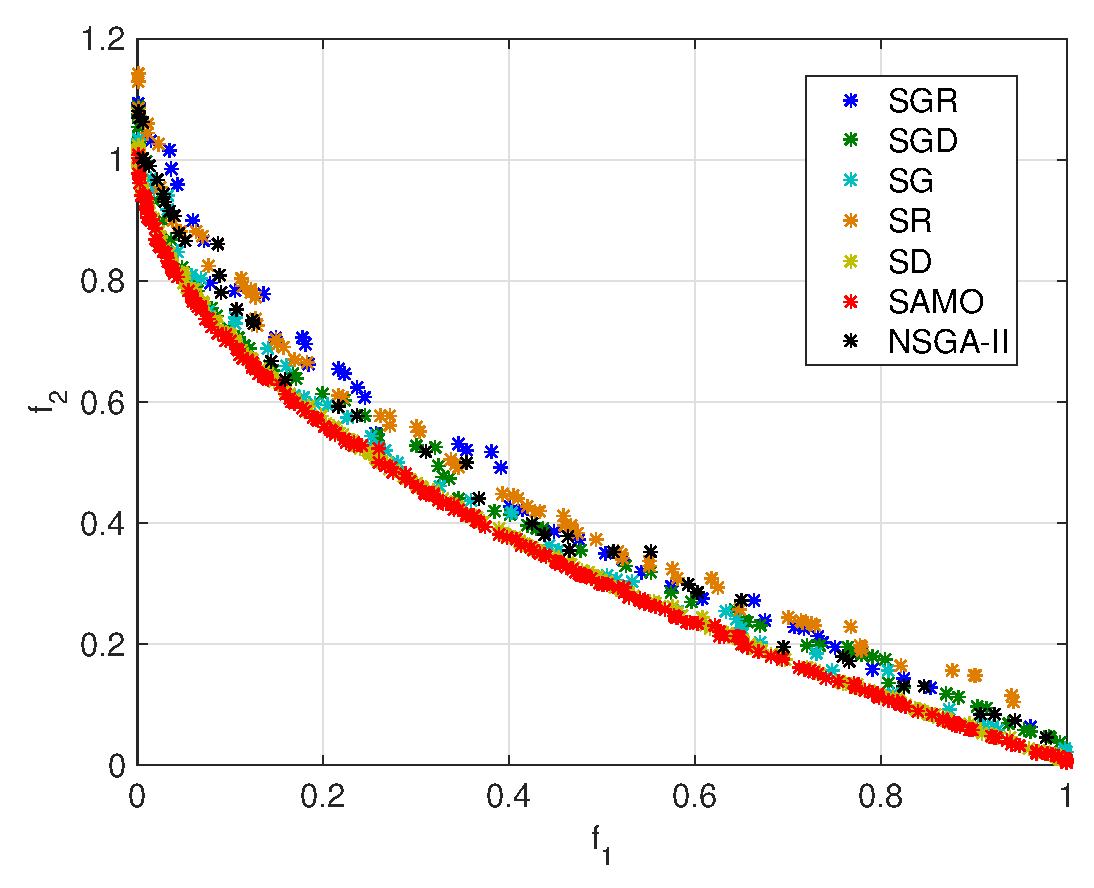
\includegraphics[scale = .21]{fig1a.eps}}
	\subfigure[]{\label{fig:c1dtlz3idbea}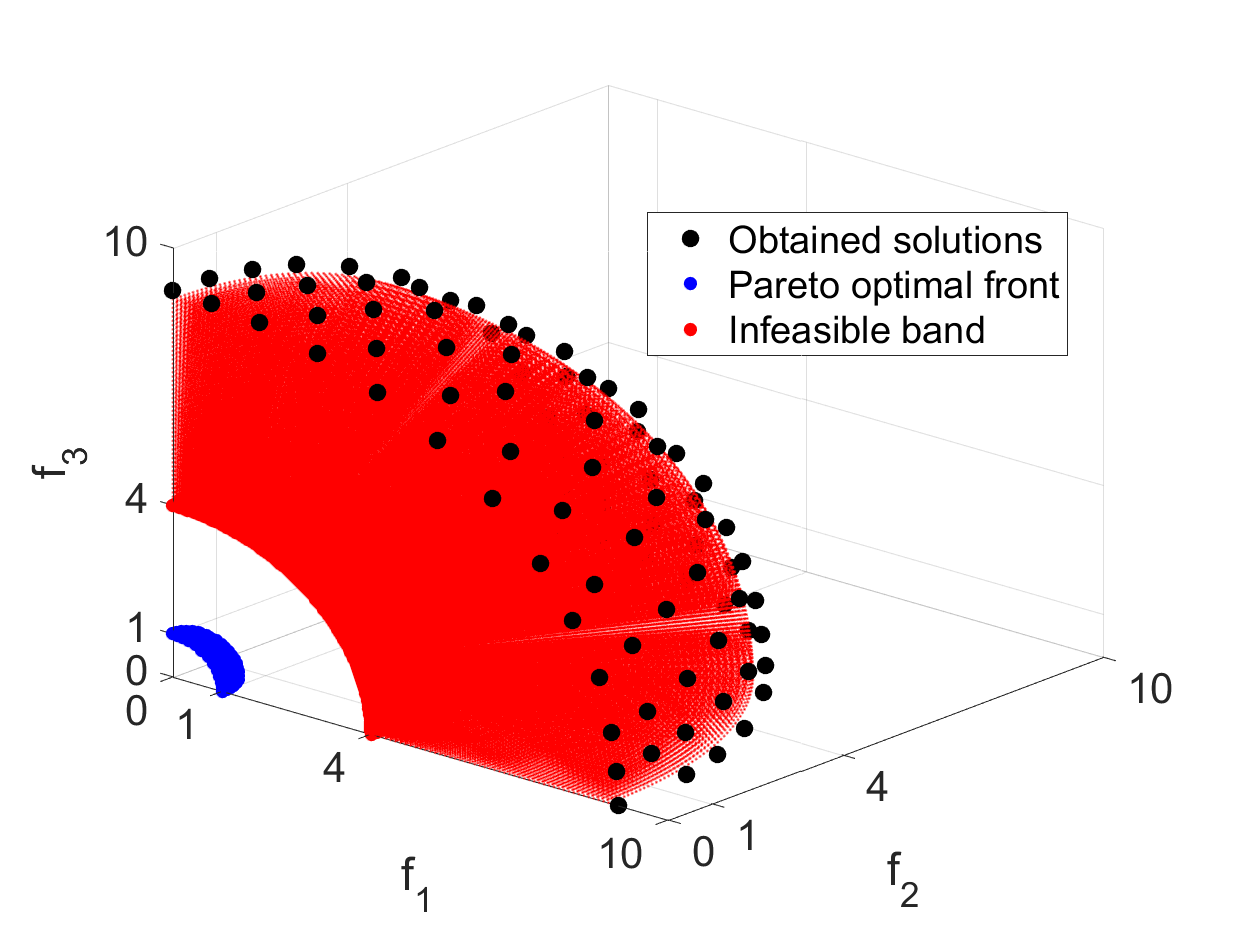
\includegraphics[scale = .21]{fig1b.eps}}
	\label{fig:rationale}
	\caption{Final distribution using I-DBEA: (a) MOP1, (b) C1DTLZ3}
\end{figure}

In this paper we aim to alleviate these issues by using a novel assignment scheme and efficient constraint handling strategy. The remainder of the paper is organized as follows. The details of the proposed algorithm are presented in Sec.~\ref{sec:algo}. The numerical experiments are presented in Sec.~\ref{sec:numex}, wherein the performance of the proposed algorithm is assessed using 4 unconstrained test problems~(3-objective DTLZ1 and DTLZ2~\cite{deb2005scalable}, 2-objective MOP1 and MOP2~\cite{liu2014mop}) and one constrained test problem~(C1DTLZ3~\cite{Deb2014adaptive}) with 3, 5 and 8 objectives. The benchmarks chosen for this paper span different class of difficulties as mentioned in \cite{liu2014mop, Wang2016adaptive}. The results are compared with the state-of-the-art approaches to establish the performance of the proposed algorithm. Thereafter, the proposed approach is used to solve a number of practical engineering design problems: a 3-objective constrained Car Side Impact (CSI) problem, a 5-objective constrained Water Resource Management~(WRM) problem, a 10-objective General Aviation Aircraft (GAA) design problem and a newly introduced 4-objective constrained Wind Farm Layout optimization problem. Sec.~\ref{sec:sum} summarizes the contributions and outlines some future research directions.


\section{Proposed Algorithm}
\label{sec:algo}

A generic multi/many-objective optimization problem can be formally defined as shown in Eqn.~\ref{eqn:MaOP}.

\begin{equation}\small
\begin{aligned}
\operatorname{Minimize}\; & f_i(\textbf{x}); i=1,2,.......M \\
\text{Subject to} & \\
& \hspace{-0.6cm}c_j(\textbf{x})\ge 0, j=1,2,.......p  \\ 
& \hspace{-0.6cm}h_j(\textbf{x}) = 0, j=1,2,.........q  \\ 
& \hspace{-0.6cm}\textbf{x}^{L}\le\textbf{x}\le\textbf{x}^{U}\\ 
\label{eqn:MaOP}
\end{aligned}
\end{equation}

\noindent Here, $f_1(\textbf{x})$  to $f_M(\textbf{x})$ are the $M$ objective functions. Without loss of generalization, minimization of each objective is assumed. The number of inequality and equality constraints are denoted by $p$ and $q$ respectively. The upper and lower bounds of the variables are denoted as $\textbf{x}^{U}$ and $\textbf{x}^{L}$ respectively. For every solution, the sum of constraint violations is denoted by $CV$, where $CV$ = $0$ indicates a feasible solution.

The proposed algorithm is based on a ($\mu$ + $\lambda$) evolutionary model, where $\mu$ parents are recombined to generate $\lambda$ offspring and the \textit{best} $\mu$ solutions are selected as parents for the next generation. The pseudo-code of the proposed method, referred to as A-DBEA~(decomposition based evolutionary algorithm with novel assignment scheme) is presented in Algorithm~\ref{alg:ADBEA}. The details of its key components are outlined in the following subsections.

\begin{algorithm}[!ht]\scriptsize
	\caption{A-DBEA}
	\textbf{Input:} $Gen_{max}$\hspace{1mm}(Maximum number of generations), $W$\hspace{1mm}(Number of Reference points/population size), Crossover and mutation parameters\\
	\begin{algorithmic}[1]
		\STATE $i$=1. \COMMENT{Generation counter}
		\STATE \textbf{Generate} $W$ reference points using Normal Boundary Intersection.
		\STATE Construct $W$ reference directions; Straight lines joining origin and $W$ reference points.
		\STATE $\theta_{th}$: Compute the minimum angle between a reference direction and all others. 
		\STATE \textbf{Initialize} the population using LHS sampling $P^{i}$; $\left|{P^{i}}\right|$ = $W$.
		\STATE \textbf{Assign} individuals of $P^{i}$ to the reference directions.
		\WHILE{$(i\le Gen_{max})$}
		\STATE \textbf{Create} $C$ offspring from $P^{i}$ via recombination.
		\STATE \textbf{Assign} $P^{i+1}$ individuals from $P^{i}+C$ to $W$ reference directions  
		\STATE $i$=$i$+1.
		\ENDWHILE
		
	\end{algorithmic}
	\label{alg:ADBEA}
\end{algorithm} 

\subsection{Generate reference directions}
\label{subsec:generate} 

A structured set of $W$ reference points is generated using the method of systematic sampling as outlined in~\cite{das1998normal}. The approach generates $W$ points on the hyperplane with a uniform spacing of $\delta=1/H$ for any number of objectives $M$ with $H$ unique sampling locations along each objective axis. The reference directions are formed by joining the ideal point~(origin in the scaled space) to each of these reference points. In this approach $N = {H+M-1}\choose{M-1}$ reference directions are generated. As discussed in \cite{Deb2014box}, one should set $H \ge M$ to obtain intermediate reference points within the simplex. However in the context of many-objective optimization involving high dimensional objective space, the number of reference points will be large even if $H = M$ (e.g. eight objective space for $H$ = 8 will result in ${8+8-1}\choose{8-1}$ = 6435 reference points). Therefore, using this approach will result in excessive number of points leading to significant computational overhead. On the other hand, increasing the spacing to achieve reduction in points results in sparsely distributed reference vectors along the boundary of the objective axes. Therefore, to overcome the above challenges, a two-layer~(referred to as $H_1$ and $H_2$) approach as suggested in \cite{Li2015dominance} is adopted which offers a means to limit the number of reference points from growing exponentially. The two-layered approach generates $N_1 = {H_1+M-1}\choose{M-1}$ points on the boundary and $N_2 = {H_2+M-1}\choose{M-1}$ points in the inside of the hyperplane. The $j^{th}$ coordinate ($W_j$) of each of the weight vectors in the inside layer generated using \cite{das1998normal} are shrunk using Eqn.~\ref{eqn:inlayer} where $\tau$ = 0.5 is considered~\cite{Li2015dominance}. An illustration is presented in Fig.~\ref{fig:Refpoint} for a 3-objective problem.

\begin{equation}
W_j = \frac{1-\tau}{M} + \tau \times W_j
\label{eqn:inlayer} 
\end{equation}   

\begin{figure}[!htb]
	\centering
	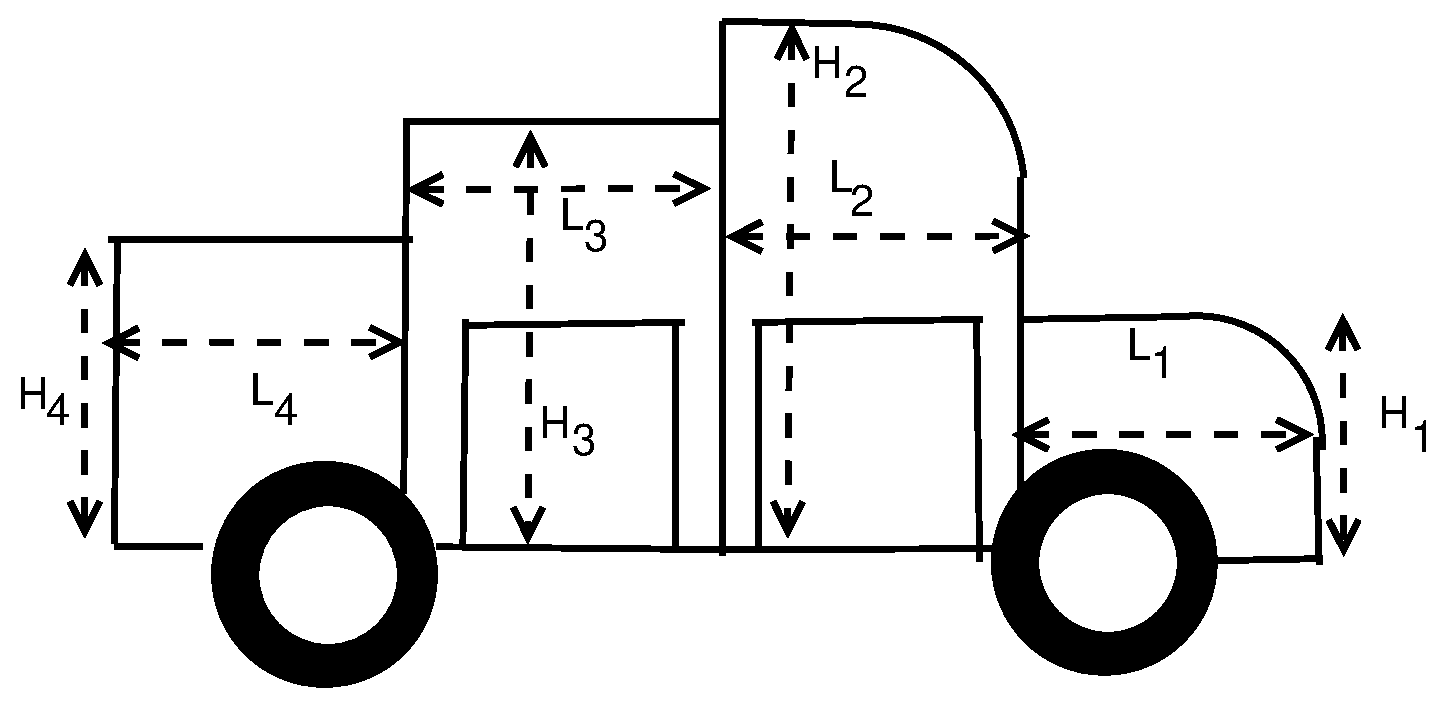
\includegraphics[width=.4\textwidth]{fig2.eps}
	\caption{Structured two-layered set of reference points with $M=3$, $H_1=1$, $H_2=1$. The filled circles represent the reference points generated on the boundary/outside layer while the hollow circles represent those generated on the inside layer.}
	\label{fig:Refpoint}
\end{figure}

\subsection{Initialize population}
\label{subsec:initialize}
The size of the population is set to be equal to the number of reference directions in this study, as is the standard practice in the domain~\cite{zhang2007moead,Li2015dominance,Deb2014box,Asafmany2015}. The solutions are initialized within the variable bounds $\textbf{x}^{L}$ and $\textbf{x}^{U}$ using Latin Hypercube Sampling based on ``maximin'' criterion.\\ 

\subsection{Assignment}
\label{subsec:assign}  

A novel scheme of is introduced to assign solutions to the reference directions in each generation. The assignment process is as follows.

The solutions in the population are first divided into two groups, feasible and infeasible. From the feasible set of solutions, the nondominated set is identified first, which is then used to compute the ideal vector~(\textbf{Z}$^I$). The vector (\textbf{Z}$^I$) is subsequently modified by subtracting a small quantity $10^{-6}$ from each of its elements, in line with the common practice~(e.g., \cite{Qi2014adaptive} and \cite{Goulart2016preference}) considered subtraction of $10^{-7}$ and $0.01$ respectively). Thereafter, nondominated solutions with minimum achievement scalarizing function~(ASF) value along each objective axis are identified as done in \cite{Yuan2016many}. The ASF, by definition, minimizes the distance from the reference point to the feasible region, if the reference point is unattainable. The reference point is considered as the ideal vector in minimization sense as stated in Eqn.~\ref{eqn:asf} for a solution $\mathbf{x}$ with respect to $i^{th}$ reference direction ($W^i$). While computing ASF values, if $W^i_j$ = 0, the value of $W^i_j$ is taken as $10^{-6}$ to eliminate division by zero, as commonly done~\cite{Yuan2016many}.

\begin{equation}
ASF(\textbf{x},W^i) = \max_{j = 1}^M \left(\frac{f_j(\textbf{x}) - Z_j^I}{W^i_j}\right)
\label{eqn:asf} 
\end{equation} 

The maximum values of the objective functions of these solutions are used to construct the nadir vector \textbf{Z}$^N$. These two vectors~(\textbf{Z}$^I$ and \textbf{Z}$^N$) are used for scaling the objective values linearly between 0 and 1. From the set of feasible solutions, the nondominated solutions with minimum ASF value along each objective axis are first assigned. For the remaining nondominated solutions, the perpendicular distances~($d_2$ as illustrated in Fig.~\ref{fig:distance_d1d2}) from each solution to all unassigned reference directions in the scaled objective space are computed. The perpendicular distance ($d_2\textbf{x}$) of a single solution ($\textbf{x}$) in the scaled objective space ($\textbf{F}_s(\textbf{x})$) to $i^{th}$ reference direction ($W^i$) can be computed using Eqn.~\ref{eqn:d2comp}, where \textbf{Z}\textsubscript{s}$^I$ is the ideal vector of the scaled objective space. $\textbf{F}_s(\textbf{x})$ is the objective vector $(f_1(\textbf{x}),\ldots, f_M(\textbf{x}))^T$ in the scaled objective space. 

\begin{equation}
d_2(\textbf{x}) = \left\vert\left\vert\textbf{F}_s(\textbf{x}) - \left({\textbf{Z}_s}^I + \frac{\left\vert\left\vert\left(\textbf{F}_s(\textbf{x}) - {\textbf{Z}_s}^I\right)^T W^i\right\vert\right\vert W^i}{{\left\vert\left\vert W^i \right\vert\right\vert}^2}\right)\right\vert\right\vert
\label{eqn:d2comp} 
\end{equation} 

\begin{figure}[!htb]
	\centering
	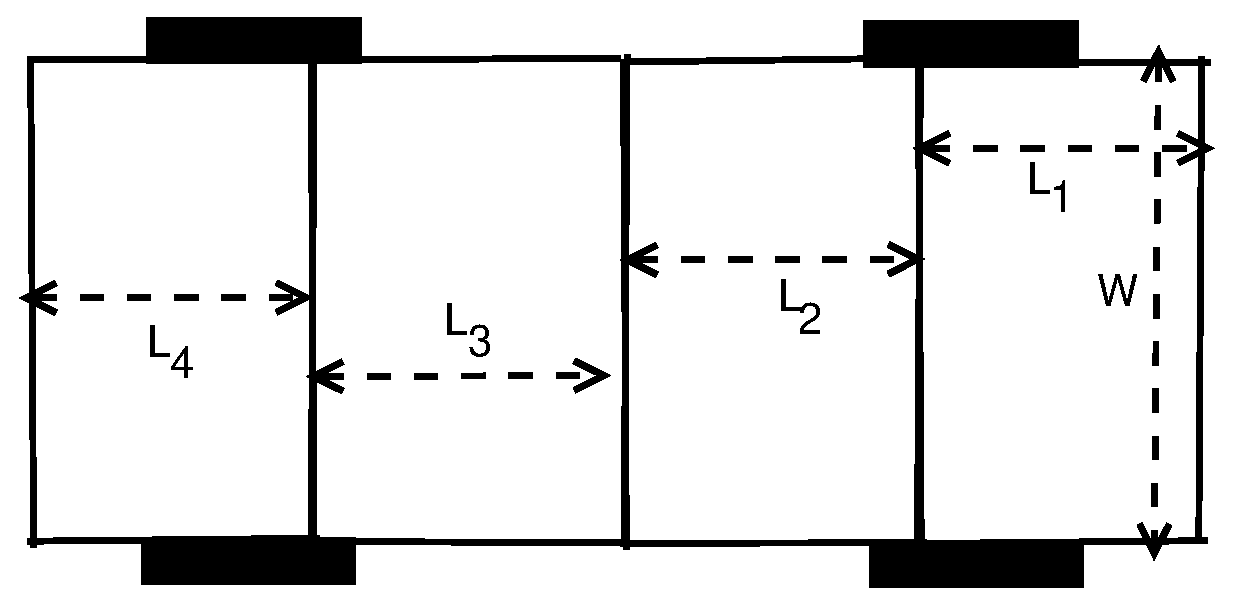
\includegraphics[scale=.3]{fig3.eps}
	\caption{$d_2$ measure}
	\label{fig:distance_d1d2}
\end{figure}

Similarly the angle value between a solution and each unassigned reference direction is also computed. A solution in the nondominated set is assigned to a reference direction via ``handshake'' if it has the least $d_2$ with that reference direction and is also the closest~(in terms of $d_2$) from that reference direction. The remaining solutions in the nondominated set are assigned using  a minimum $d_2$ based criterion, where reference directions are selected in a random order to avoid any bias. If such an assignment results in an angle value~(between a solution and its assigned reference direction) being more than a threshold $\theta_{th}$, the solution is discarded and the reference direction is made available to the assignment process in the next nondominated front as shown in Fig.~\ref{fig:assignmentnd}. The value of $\theta_{th}$ for any given reference direction is the minimum of all the angles it forms with all other reference directions.

The above process is repeated for each subsequent front. After the process has been completed for all fronts, some unassigned reference directions might still remain~(as a result of discarded solutions previously assigned to this direction). If so, the remaining solutions are sorted based on nondominance and the same scheme of ``handshake'' and minimum $d_2$ based assignment is performed without the $\theta_{th}$ considerations.

If the number of feasible solutions is less than $W$, some unassigned directions will still remain after above process. In such cases, there is a need to select infeasible solutions. The infeasible solutions are sorted based on ascending order of their sum of constraint violation measure. If there are $c$ unassigned reference directions, top $c$ infeasible solutions are selected for assignment. The objective values of these $c$ solutions are normalized between $0$ and $1$. The perpendicular distances~($d_2$) from each infeasible solution to $c$ unassigned reference directions are calculated in the normalized objective space. An infeasible solution is assigned to a reference direction via ``handshake''and minimum~$d_2$ based criterion similar to the process discussed above.

\begin{figure}[!htb]
	\centering
	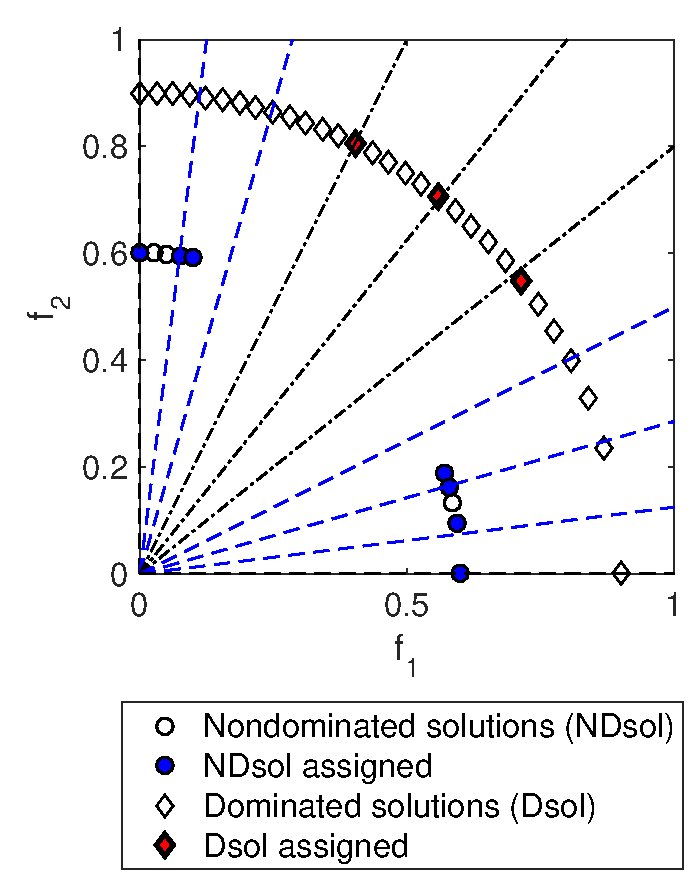
\includegraphics[scale=.4]{fig4.eps}
	\caption{Assignment strategy}
	\label{fig:assignmentnd}
\end{figure}

\subsection{Create offspring solutions}
\label{subsec:create} 

The process of offspring creation involves two steps, identification of participating parents for recombination and the recombination process itself. Both these steps are known to affect the performance and various rationales and recommendations have been suggested in the literature. 

Let us first consider the first case where all individuals in the population are feasible. In this case each solution is selected as a base parent and two partners are randomly chosen from a given neighborhood size~(set to 20 in this study) of closest reference directions with a high probability of $\delta = 0.9$. Otherwise participating parents will be selected from the pool of all solutions. Such a scheme offers opportunity to all solutions to act as base parents for generating offspring, while for each crossover, the neighboring directions have higher probability to recombine.

Next, let us consider the second case where a population contains a mix of feasible and infeasible solutions. Most algorithms adopt a feasible first strategy, i.e., feasible solutions are ranked explicitly above the infeasible solutions. Among the feasible solutions, the solutions are ordered by fronts and within a front, the extremal solutions are at the top followed by the remaining ones typically based on a diversity measure. With the above ordered set of solutions, a binary tournament can be performed to identify the set of $\mu$ participating parents. Such a scheme was adopted in nondominated sorting generic algorithm~(NSGA-II)~\cite{deb2002fast} and has been very successful in dealing with a range of problems. However, ranking all feasible solutions above all infeasible solutions in the ordered list has important implications\cite{Ray2009idea,Singh2013idea}. Ideally, a marginally infeasible solution might be closer to the true optimum, which often lies on a constraint boundary, and allowing participation of such solutions would be more beneficial than using a feasible solution away from the true optimum, as investigated in a number of recent studies~\cite{singh2016use}. An ordering scheme which places marginally infeasible solutions at the top of the ranked list of solutions appears in \cite{Ray2009idea}. The same scheme has been used in the proposed approach to order the solutions which subsequently engage in a binary tournament resulting in a set of $\mu$ base parents. It is important to highlight that preservation marginally infeasible solutions is known to significantly improve the rate of convergence of optimization algorithms as reviewed in \cite{singh2016use}. Two participating parents for each base parent are identified in the same way as it was for the first case. 

In order to utilize the advantages of both differential evolution~(DE) crossover~\cite{das2011de} and simulated binary crossover~(SBX)~\cite{deb2002fast}, at each generation both types of crossover are employed for alternate base parents. Similarly during the evolution, reverse order of crossover types are used in alternate generations. Thus, if in generation 1, first reference direction uses DE crossover and second reference direction uses SBX crossover, then in generation 2 the first reference direction will use SBX and the second will use DE crossover. The intent is to improve convergence by adopting the high quality solutions generated using the two crossovers, while also avoiding bias towards either of them. 

\subsection{Performance Metrics}

Inverted generation distance~(IGD) and hypervolume~(HV) are the most common metrics used for an quantitative assessment in the multiobjective optimization domain. It is important to highlight that neither of them are foolproof. Computation of IGD requires a reference Pareto front, while computation of HV requires a reference point. The reference Pareto front is usually not available for problems with unknown or complex Pareto fronts such as the engineering design optimization problems discussed later in the paper. The aspect of ``uniformity'' of solutions in the reference set is arguable and results delivered by methods which do not use reference directions such as HypE~\cite{bader2011hype} cannot be fairly compared. As for HV, the choice of the reference point used during computation is crucial and can significantly influence the interpretations about relative performance~\cite{auger2009theory,Yuan2016many,ishibuchi2010many}. 

For HV computation, recent studies suggest use of slightly larger objective values for a reference point than those of the nadir vector~\cite{auger2009theory,Yuan2016many,ishibuchi2010many}. In our experiments, we have used the reference point to be 1.1 multiplied by the true nadir vector~\cite{Yuan2016many} for problems where the nadir vector is theoretically known/analytically computed. Given a set of solutions and their corresponding objective vectors, we first discard all solutions that do not dominate the reference point. The objective vectors of the remaining solutions are normalized using the ideal and the nadir vector listed in Table \ref{tab:prob_param} and HV is computed using a reference point as $1.1^M$~\cite{Yuan2016many}, where $M$ is the number of objectives. All HV computations are done using WFG algorithm reported in \cite{while2012hv}. 

HV and IGD computations in this paper are based on solutions obtained from the archive (set of all fully evaluated solutions so far) instead of the final population obtained at the end of optimization. At first all the nondominated solutions are collected from the archive. In the next stage, for each reference direction, the solution closest based on $d_2$ measure is selected. The exceptions~(to the use of archive) are the Water Resource Management, as there are a large number of nondominated points in the archive. For this problem, the nondominated solutions in the final population have been used for HV and IGD computations.  

\begin{table*}\scriptsize
	\centering
	\caption{Details of the problems studied}
	\label{tab:prob_param}
	\begin{tabular}{|l|l|p{3cm}|p{3cm}|p{3cm}|p{4cm}|}
		\noalign{\smallskip}\hline
		\textbf{Problem}            & \textbf{M} & \textbf{Ideal Point}                             & \textbf{nadir Point}                                                    & \textbf{Number of Variables}                         & \textbf{Range of Variables}             \\ \hline
		DTLZ1										& 3          & (0, 0, 0)                 & (0.5, 0.5, 0.5)                                                & M+k-1 (M = 3, k = 5)                                & {[}0, 1{]}, ($\forall$ i = 1,\dots 7)  \\ \hline
		DTLZ2										& 3          & (0, 0, 0)                 & (1, 1, 1)                                                & M+k-1 (M = 3, k = 10)                                & {[}0, 1{]}, ($\forall$ i = 1,\dots 12)  \\ \hline
		MOP1										& 2          & (0, 0)                 & (1, 1)                                                & 10                               & {[}0, 1{]}, ($\forall$ i = 1,\dots 10)  \\ \hline
		MOP2										& 2          & (0, 0)                 & (1, 1)                                                & 10                               & {[}0, 1{]}, ($\forall$ i = 1,\dots 10)  \\ \hline
		& 3          & (0, 0, 0)                                        & (1, 1, 1)                                                         & M+k-1 (M = 3, k = 10)                                 & {[}0, 1{]}, ($\forall$ i = 1,\dots 12)   \\ \cline{2-6}
		C1DTLZ3                     & 5          & (0, 0, 0, 0, 0)                                  & (1, 1, 1, 1, 1)                                               & M+k-1 (M = 5, k = 10)                                 & {[}0, 1{]}, ($\forall$ i = 1,\dots 14)   \\ \cline{2-6}
		& 8          & (0, 0, 0, 0, 0, 0, 0, 0)                         & (1, 1, 1, 1, 1, 1, 1, 1)                                & M+k-1 (M = 8, k = 10)                                 & {[}0, 1{]}, ($\forall$ i = 1,\dots 17)  \\ \hline
		CSI										& 3          & (23.5895, 3.5852, 10.6106)                 & (42.7680, 3.9999, 12.5211)                                                & 7                                & $x^{L}$ = [0.5,0.45,0.5,0.5,0.875,0.4,0.4], $x^{U}$ = [1.5,1.35,1.5,1.5,2.625,1.2,1.2]  \\ \hline
		WRM										& 5          & (63840.2774, \textbf{44.5836}, 285346.8965, 183749.9671, 7.2222)                 & (\textbf{73709.9433}, 1350.0000, 2853468.9650, \textbf{6601771.4635}, \textbf{24998.3176})                                                & 3                                & $x^{L}$ = [0.01,0.01,0.01], $x^{U}$ = [0.45,0.10,0.10]  \\ \hline
		GAA                   & 10          & (73.2507, 1881.4729, 59.1141, 1.7977, 359.9166, 41878.8363, -2580.1544, -16.8232, -204.0244, 0.2685)                 & (\textbf{74.0784}, 2011.4952,79.9930, 2.0000, \textbf{493.9002}, 44590.1399, -2000.0017, -14.4082, -189.2993, \textbf{2.3507})                                                & Please refer to problem description                                & Please refer to problem description  \\ \hline
	\end{tabular}
\end{table*}


\section{Numerical Experiments}
\label{sec:numex}

\subsection{Experimental Settings}

The parameter settings and benchmarking process presented here comply with prior studies\cite{Deb2014adaptive,Wang2016adaptive} for a fair comparison. A probability of crossover of 1 and a probability of mutation of $\frac{1}{n}$ ($n$ is the number of variables)~\cite{Deb2014adaptive} was used for all problems. The distribution index of crossover and mutation was set to 30 and 20 respectively~\cite{Deb2014adaptive}. The crossover rate ($CR$) and scaling factor ($F$) are set as 1 and 0.5 respectively for the DE crossover as recommended in~\cite{das2011de}. The infeasibility ratio~(for the infeasibility driven constraint handling scheme) was set to 0.20, i.e, 20\% marginally infeasible solutions are ranked above the feasible solutions as suggested in \cite{Singh2013idea}.  The formulations of the problems considered in this study are available for download from the author's website~\cite{mdo2017adbea} and are not presented here for brevity. Full default precision of MATLAB has been used without any rounding/casting~\footnote{The results obtained by MaO algorithms may also depend on this aspect. Rounding the objective values to certain digits might offer unfair advantages for some cases.}. The problem-specific settings used are as follows:

\begin{enumerate}
	\item \textit{Population Size}: The population size is set as 300~\cite{Wang2016adaptive} for 3-objective DTLZ1 and DTLZ2~($H$ = 23),  and 2-objective MOP1 and MOP2~($H$ = 299). For C1DTLZ3~\cite{Deb2014adaptive}, the population size for 3-objective instance is 91 ($H$ = 12), 5-objective instance is 210 ($H$ = 6) and 8-objective instance is 156 ($H_1$ = 3, $H_2$ = 2). For the engineering design examples, the population size for 3-objective Car Side Impact problem~\cite{Deb2014adaptive} is 153 ($H$ = 16), 5-objective Water Resource Management~\cite{Asafmany2015} is 210 ($H$ = 6), 10-objective General Aviation Aircraft design~\cite{Asafmany2015} is 275 ($H_1$ = 3, $H_2$ = 2) and 4-objective Wind Farm Layout optimization is 220~($H$ = 9).
	\item \textit{Stopping Condition}: The maximum number of function evaluations are set to be 100,000 for DTLZ1 and DTLZ2 problems~\cite{Wang2016adaptive}, 300,000 for MOP1 and MOP2 problems~\cite{Wang2016adaptive}, 91,000 for 3-objective instance of C1DTLZ3~\cite{Deb2014adaptive}, 315,000 for 5-objective instance\cite{Li2015dominance}, 390,000 for 8-objective instance~\cite{Li2015dominance}, 76,500 for the Car Side Impact problem~\cite{Deb2014adaptive}, 210,000 for Water Resource Management problem\cite{Asafmany2015}, 275,000 for General Aviation Aircraft design problem and 88,000 for Wind Farm Layout optimization problem.
	\item Number of independent optimization runs is set to be 30 for the DTLZ1, DTLZ2, MOP1 and MOP2 problems~\cite{Wang2016adaptive}, and 21 for the C1DTLZ3, Car Side Impact, Water Resource Management and General Aviation Aircraft design problems. These numbers have been chosen to compare the results obtained using the proposed approach with results from same number of runs used in previous studies. For the newly formulated Wind Farm Layout optimization problem, there are no existing results to compare with, and we present and analyze results obtained from a single run.
	\item The performance of I-DBEA~\cite{Asafmany2015} on all problems was studied based on the same experimental settings as adopted for A-DBEA. The code of I-DBEA was obtained from the authors to execute these experiments.  
\end{enumerate}

The results of numerical experiments are discussed next, organized into three parts: unconstrained test problems, constrained test problem, and engineering design problems. 

\subsection{Unconstrained Test Problems}

The performance of A-DBEA for unconstrained DTLZ1, DTLZ2, MOP1 and MOP2 problems in terms of HV measure~(Best, Mean, Median and Worst) is presented in Table~\ref{tab:hvunc} and compared with I-DBEA. While I-DBEA performs better for DTLZ1, A-DBEA performs significantly better in others. Since approaches relying on global nondominance during replacement are known to be effective for DTLZ1, I-DBEA performs better than the proposed approach. To the best of authors' knowledge, the HV statistics of these problems are not presented elsewhere. Fig.~\ref{fig:frontunc} presents the nondominated solutions obtained using A-DBEA for the runs with best (i.e. minimum) IGD value. 

\begin{table}[!htb]\scriptsize
	\centering
	\caption{HV statistics~(from the top: best, mean, median, worst) for the unconstrained problems}
	\label{tab:hvunc}
	\tabcolsep = 0.05cm
	\begin{tabular}{|c|c|c|c|c|c|c|c|}
		\noalign{\smallskip}\hline
		\multicolumn{2}{|c|}{\textbf{DTLZ1}} & \multicolumn{2}{c|}{\textbf{DTLZ2}}   & \multicolumn{2}{c|}{\textbf{MOP1}}  & \multicolumn{2}{c|}{\textbf{MOP2}}  \\ \hline
		\textbf{A-DBEA}  & \textbf{I-DBEA}   & \textbf{A-DBEA}   & \textbf{I-DBEA}   & \textbf{A-DBEA}   & \textbf{I-DBEA} & \textbf{A-DBEA}   & \textbf{I-DBEA} \\ \hline
		1.118872         & \textbf{1.141377} & 0.773105          & \textbf{0.773472} & \textbf{0.853143} & 0.323468        & \textbf{0.537582} & 0.210000        \\
		1.016394         & \textbf{1.135242} & \textbf{0.772734} & 0.771297          & \textbf{0.851319} & 0.313001        & \textbf{0.536911} & 0.210000        \\
		1.051432         & \textbf{1.139191} & \textbf{0.772787} & 0.771664          & \textbf{0.851442} & 0.312540        & \textbf{0.536891} & 0.210000        \\
		0.716614         & \textbf{1.072950} & \textbf{0.772161} & 0.768711          & \textbf{0.849320} & 0.298565        & \textbf{0.536229} & 0.210000        \\ \hline
	\end{tabular}
\end{table}

\begin{table*}[!htb]\scriptsize
	\centering
	\caption{IGD statistics~(from the top: best, mean, median, worst) for unconstrained problems}
	\label{tab:IGDunc}
	\tabcolsep = 0.1cm
	\begin{tabular}{|l|l|l|l|l|l|l|l|l|l|l|}
		\noalign{\smallskip}\hline
		\textbf{Problem} & \textbf{A-DBEA}      & \textbf{I-DBEA}         & \textbf{NSGA-III} & \textbf{SMS-EMOA} & \textbf{MOEA/D-DE} & \textbf{ENS-MOEA/D} & \textbf{MOEA/D-M2M} & \textbf{MOEA/D-GR} & \textbf{MOEA/D-AGR} & \textbf{gMOEA/D-AGR} \\ \hline
		\textbf{DTLZ1}   & 3.42E-02 & \textbf{2.07E-02}    & $--$             & $--$              & 6.90E-02           & $--$                & $--$                & 4.47E-02           & 4.29E-02            & $--$                 \\ \cline{2-11} 
		\textbf{}        & 9.58E-02 & \textbf{2.43E-02}    & 3.26E-01         & 2.87E-01          & 4.85E-01           & 2.99E-01            & 1.62                & 2.59E-01           & 2.66E-01            & 2.87E-01             \\ \cline{2-11} 
		\textbf{}        & 7.83E-02 & \textbf{2.14E-02}    & $--$             & $--$              & 3.01E-01           & $--$                & $--$                & 2.57E-01           & 2.61E-01            & $--$                 \\ \cline{2-11} 
		\textbf{}        & 2.26E-01          & \textbf{6.03E-02}    & $--$             & $--$              & $--$               & $--$                & $--$                & $--$               & $--$                & $--$                 \\ \hline
		\textbf{DTLZ2}   & \textbf{2.67E-02} & 2.68E-02    & $--$             & $--$              & 2.82E-02           & $--$                & $--$                & 2.82E-02           & 2.80E-02            & $--$                 \\ \cline{2-11} 
		\textbf{}        & \textbf{2.69E-02} & 2.71E-02    & 3.97E-02         & 7.07E-01          & 2.87E-02           & 3.73E-02            & 4.33E-02            & 2.87E-02           & 2.84E-02            & 2.84E-02             \\ \cline{2-11} 
		\textbf{}        & \textbf{2.69E-02} & 2.70E-02    & $--$             & $--$              & 2.88E-02           & $--$                & $--$                & 2.86E-02           & 2.84E-02            & $--$                 \\ \cline{2-11} 
		\textbf{}        & 2.78E-02          & 2.90E-02    & $--$             & $--$              & $--$               & $--$                & $--$                & $--$               & $--$                & $--$                 \\ \hline
		\textbf{MOP1}    & \textbf{1.67E-02} & 3.50E-01    & $--$             & $--$              & 1.59E-01           & $--$                & $--$                & 1.70E-02           & 1.71E-02            & $--$                 \\ \cline{2-11} 
		\textbf{}        & \textbf{1.78E-02} & 3.54E-01    & 3.55E-01         & 2.84E-01          & 3.13E-01           & 4.41E-01            & 2.65E-02            & 2.10E-02           & 2.14E-02            & 2.07E-02             \\ \cline{2-11} 
		\textbf{}        & \textbf{1.77E-02} & 3.55E-01    & $--$             & $--$              & 3.52E-01           & $--$                & $--$                & 1.99E-02           & 1.99E-02            & $--$                 \\ \cline{2-11} 
		\textbf{}        & 1.94E-02          & 3.60E-01    & $--$             & $--$              & $--$               & $--$                & $--$                & $--$               & $--$                & $--$                 \\ \hline
		\textbf{MOP2}    & 3.30E-03          & 3.54E-01    & $--$             & $--$              & 1.74E-01           & $--$                & $--$                & 3.30E-03           & \textbf{2.80E-03}   & $--$                 \\ \cline{2-11} 
		\textbf{}        & \textbf{3.70E-03} & 3.54E-01    & 3.47E-01         & 3.54E-01          & 3.06E-01           & 3.11E-01            & 9.87E-03            & 6.37E-02           & 4.42E-02            & 5.52E-02             \\ \cline{2-11} 
		\textbf{}        & \textbf{3.80E-03} & 3.54E-01    & $--$             & $--$              & 3.54E-01           & $--$                & $--$                & 1.61E-02           & 7.2E-03             & $--$                 \\ \cline{2-11} 
		\textbf{}        & 4.20E-03          & 3.54E-01    & $--$             & $--$              & $--$               & $--$                & $--$                & $--$               & $--$                & $--$                 \\ \hline               
	\end{tabular}
\end{table*}																								



\begin{figure*}[!htb]
	\centering
	\subfigure[]{\label{fig:dtlz1}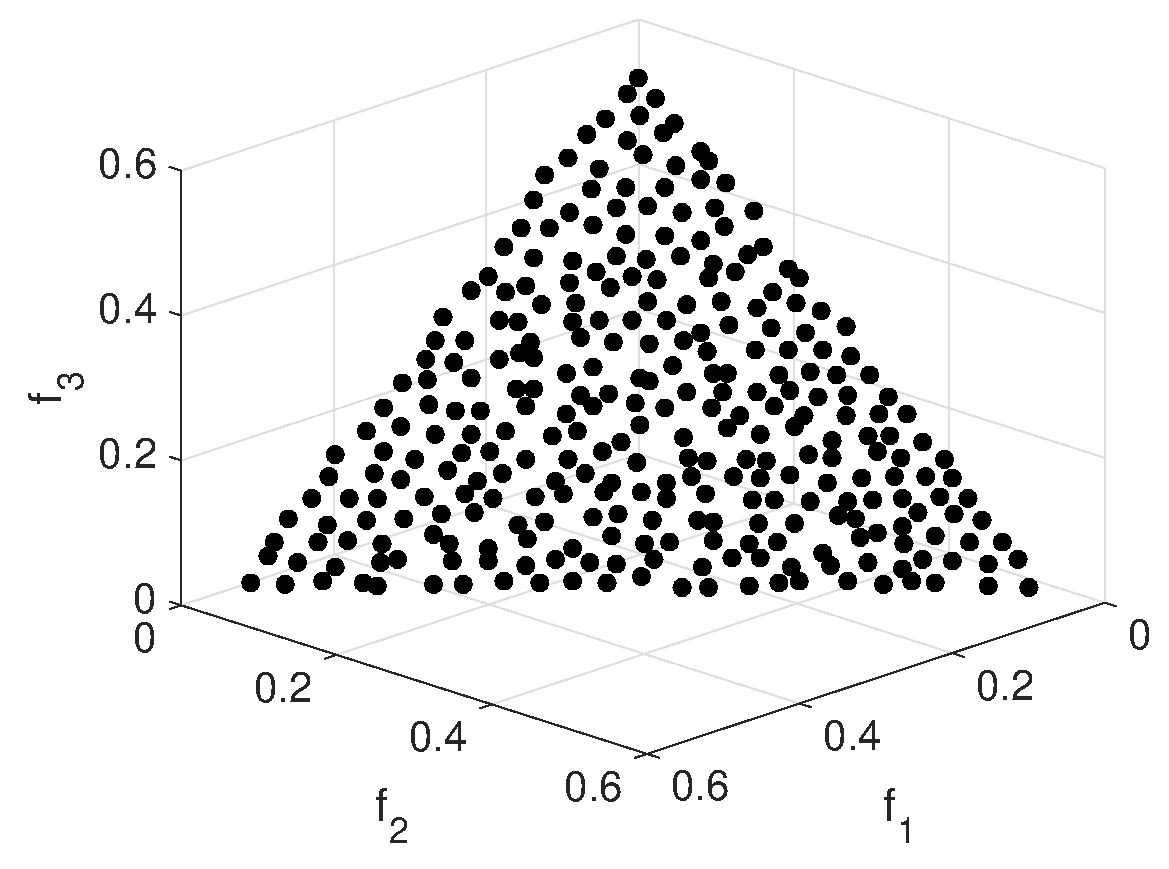
\includegraphics[scale=.21]{fig5a.eps}}
	\subfigure[]{\label{fig:dtlz2}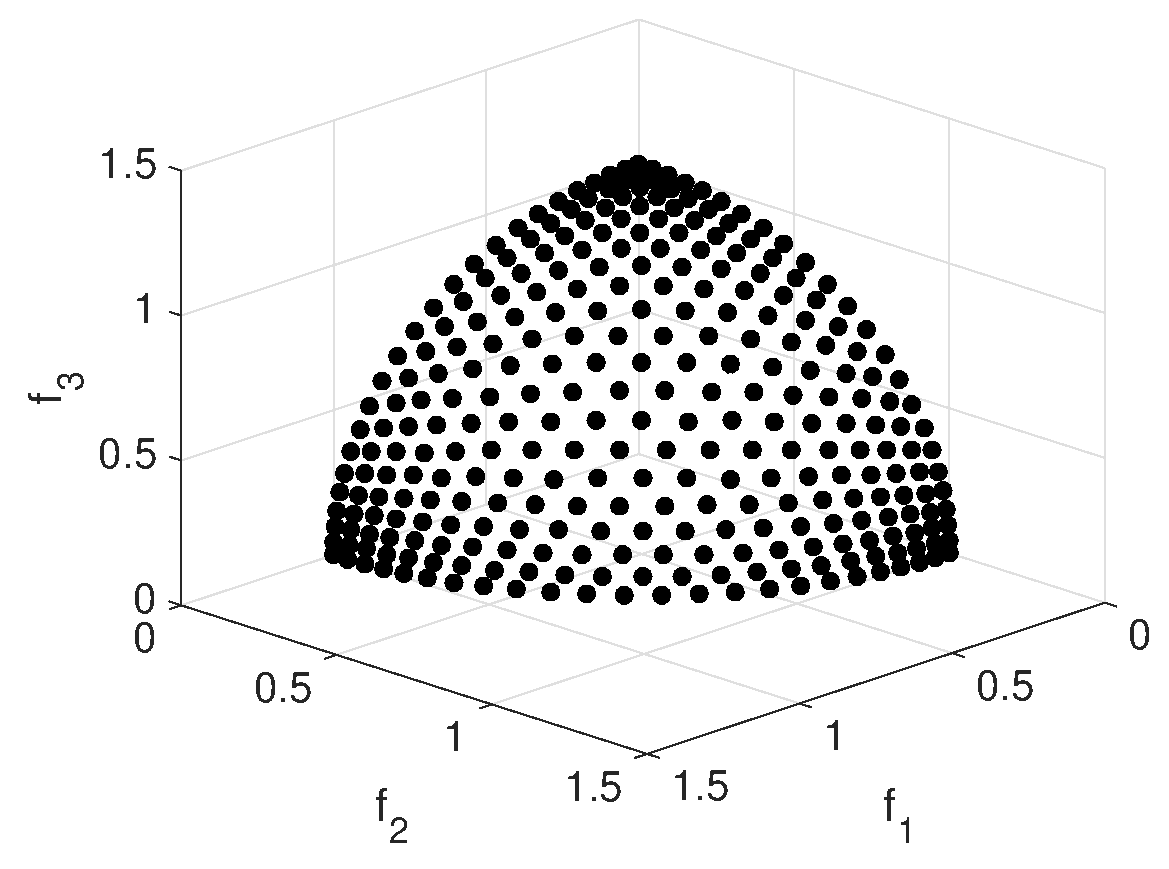
\includegraphics[scale=.21]{fig5b.eps}}
	\subfigure[]{\label{fig:mop1}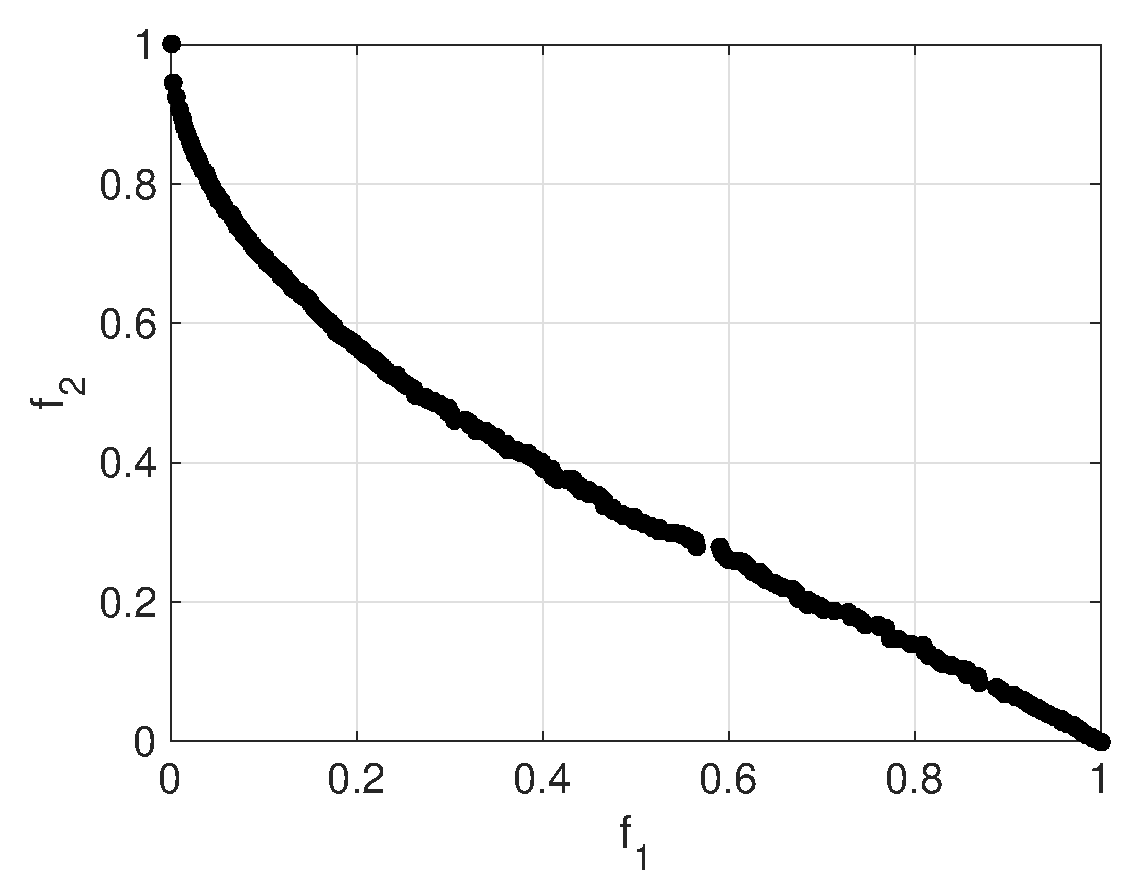
\includegraphics[scale=.21]{fig5c.eps}}
	\subfigure[]{\label{fig:mop2}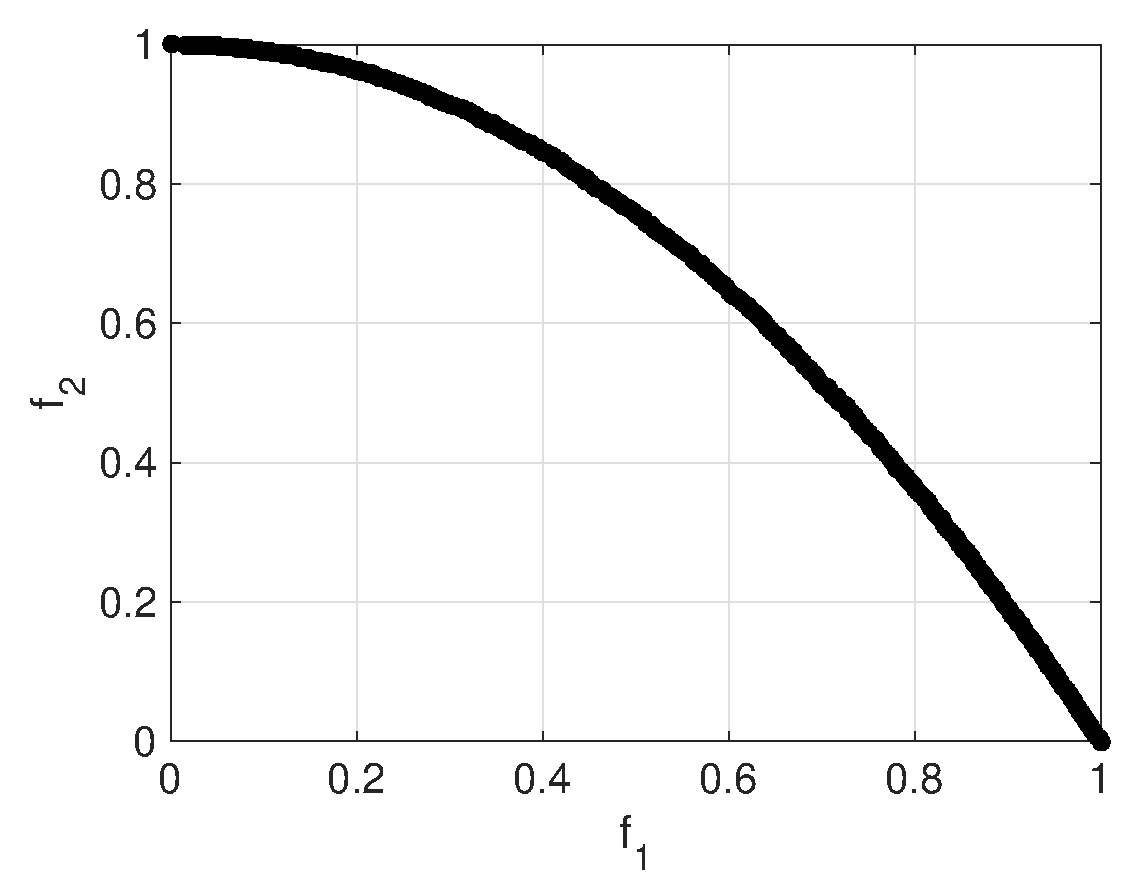
\includegraphics[scale=.21]{fig5d.eps}}
	\caption{Nondominated solutions for the runs with the lowest IGD values for unconstrained problems obtained using A-DBEA: (a) DTLZ1, (b) DTLZ2, (c) MOP1 and (d) MOP2}
	\label{fig:frontunc}
\end{figure*}

Next, the performance of A-DBEA is presented in terms of IGD measure~(best, mean, median and worst) for each unconstrained problem in order to benchmark with those reported in \cite{Wang2016adaptive}. The results are presented and compared with I-DBEA~\cite{Asafmany2015}, NSGA-II~\cite{deb2002fast}, SMS-EMOA~\cite{beume2007sms}, MOEA/D-DE~\cite{li2009multiobjective}, ENS-MOEA/D~\cite{zhao2012ens}, MOEA/D-M2M~\cite{liu2014mop}, MOEA/D-GR~\cite{Wang2016adaptive}, MOEA/D-AGR~\cite{Wang2016adaptive} and gMOEA-D/AGR~\cite{Wang2016adaptive} in Table~\ref{tab:IGDunc}. Large number of solutions in the reference set could measure both convergence and diversity as discussed in \cite{Wang2016adaptive}. Therefore, the number of solutions in the reference set is kept as 1000 for DTLZ1 and DTLZ2 and 500 for MOP1 and MOP2. Best IGD values for various statistics are marked in bold in Table\ref{tab:IGDunc}. For DTLZ1 problem, I-DBEA performs best in terms of best, mean, median and worst IGD statistics since global nondominance during replacement is known to be effective for this problem. For other problems, A-DBEA performs better than all the other algorithms. 

\subsection{Constrained Test Problem}

We now investigate the performance of A-DBEA on a representative constrained test problem, introduced in \cite{Deb2014adaptive}. The performance of A-DBEA in terms of HV is shown in Table~\ref{tab:hvigdc} and compared with I-DBEA. It is evident that performance of A-DBEA is significantly better compared to I-DBEA due to efficient constraint handling strategy. To the best of our knowledge, there are no reports on HV for these problems based on other algorithms. Hence our comparison is based on IGD, presented in Table~\ref{tab:hvigdc}. In terms of HV comparison, none of the runs of I-DBEA could obtain solutions that dominate the true nadir point for this problem. Hence the HV values of the nondominated solutions obtained using I-DBEA are zero. 

\begin{table}[!htb]\scriptsize
	\centering
	\caption{HV and IGD statistics~(best, mean, median, worst) for the constrained problem C1DTLZ3}
	\label{tab:hvigdc}
	\tabcolsep = 0.1cm
	\begin{tabular}{|c|c|c|c|c|c|c|}
		\noalign{\smallskip}\hline
		\textbf{}  & \multicolumn{2}{c|}{\textbf{HV}}    & \multicolumn{4}{c|}{\textbf{IGD}}                                                \\ \hline
		\textbf{M} & \textbf{A-DBEA}   & \textbf{I-DBEA} & \textbf{A-DBEA}   & \textbf{I-DBEA} & \textbf{C-NSGA-III}    & \textbf{C-MOEA/D} \\ \hline
		\textbf{3} & \textbf{0.744079} & 0.000000        & 3.00E-03          & 8.00            & 8.65E-04               & \textbf{4.40E-04} \\
		& \textbf{0.743117} & 0.000000        & \textbf{4.40E-03} & 8.01            & $--$                   & $--$              \\
		& \textbf{0.743232} & 0.000000        & \textbf{4.30E-03} & 8.01            & 8.14E-03 (13)          & $--$ (8)          \\
		& \textbf{0.741191} & 0.000000        & \textbf{6.70E-03} & 8.02            & $--$ (13)              & $--$ (8)          \\ \hline
		\textbf{5} & \textbf{1.075225} & 0.000000        & 3.19E-01          & 11.56           & 1.03E-03               & \textbf{2.65E-04} \\
		& \textbf{1.016748} & 0.000000        & \textbf{3.57E-01} & 11.59           & $--$                   & $--$              \\
		& \textbf{1.023992} & 0.000000        & 3.57E-01          & 11.59           & \textbf{5.10E-02 (15)} & $--$ (8)          \\
		& \textbf{0.912324} & 0.000000        & \textbf{3.91E-01} & 11.64           & $--$ (15)              & $--$ (8)          \\ \hline
		\textbf{8} & \textbf{1.870341} & 0.000000        & 3.33E-01          & 12.32           & \textbf{1.66E-03}      & 5.00E-01          \\
		& \textbf{1.807792} & 0.000000        & \textbf{3.85E-01} & 12.35           & $--$                   & $--$              \\
		& \textbf{1.813639} & 0.000000        & 3.89E-01          & 12.35           & \textbf{1.20E-02 (14)} & $--$ (1)          \\
		& \textbf{1.645524} & 0.000000        & \textbf{4.13E-01} & 12.35           & $--$ (14)              & $--$ (1)          \\ \hline
	\end{tabular}
\end{table}	

The IGD results~(computed in the same way as \cite{Li2015dominance}) are compared with I-DBEA~\cite{Asafmany2015}, C-NSGA-III~\cite{Deb2014adaptive} and C-MOEA/D~\cite{Deb2014adaptive} in Table~\ref{tab:hvigdc}. Studies on the test problem C1DTLZ3 have been scarcely reported in literature. It is particularly challenging as the Pareto front is enclosed by a layer of infeasible region. As reported in \cite{Deb2014adaptive}, out of 20 runs, NSGA-III could only reach the Pareto front in 13, 15 and 14 runs across 3, 5 and 8 objective problems respectively, while C-MOEA/D did so in even fewer runs, i.e., 8, 8 and 1~(indicated in brackets in Table~\ref{tab:hvigdc}). Although all the solutions in the final population obtained using I-DBEA are feasible, the IGD values of these solutions are significantly worse than the proposed approach. This can be accounted for having a poor constraint handling strategy and it fails to penetrate the infeasible layer~\cite{Deb2014adaptive} near the Pareto optimal front. The proposed algorithm however reached the Pareto front in all 21 runs across all objective problems. While the best run has lower IGD using C-MOEA/D, the overall statistics are better for all 3,5,8 objective versions of this problem using A-DBEA. Fig.~\ref{fig:frontc} shows the nondominated solutions with the lowest IGD values for the 3-objective C1DTLZ3. This example clearly highlights the consistent and reliable performance of the proposed approach for constrained problems.

\begin{figure}[!htb]
	\centering
	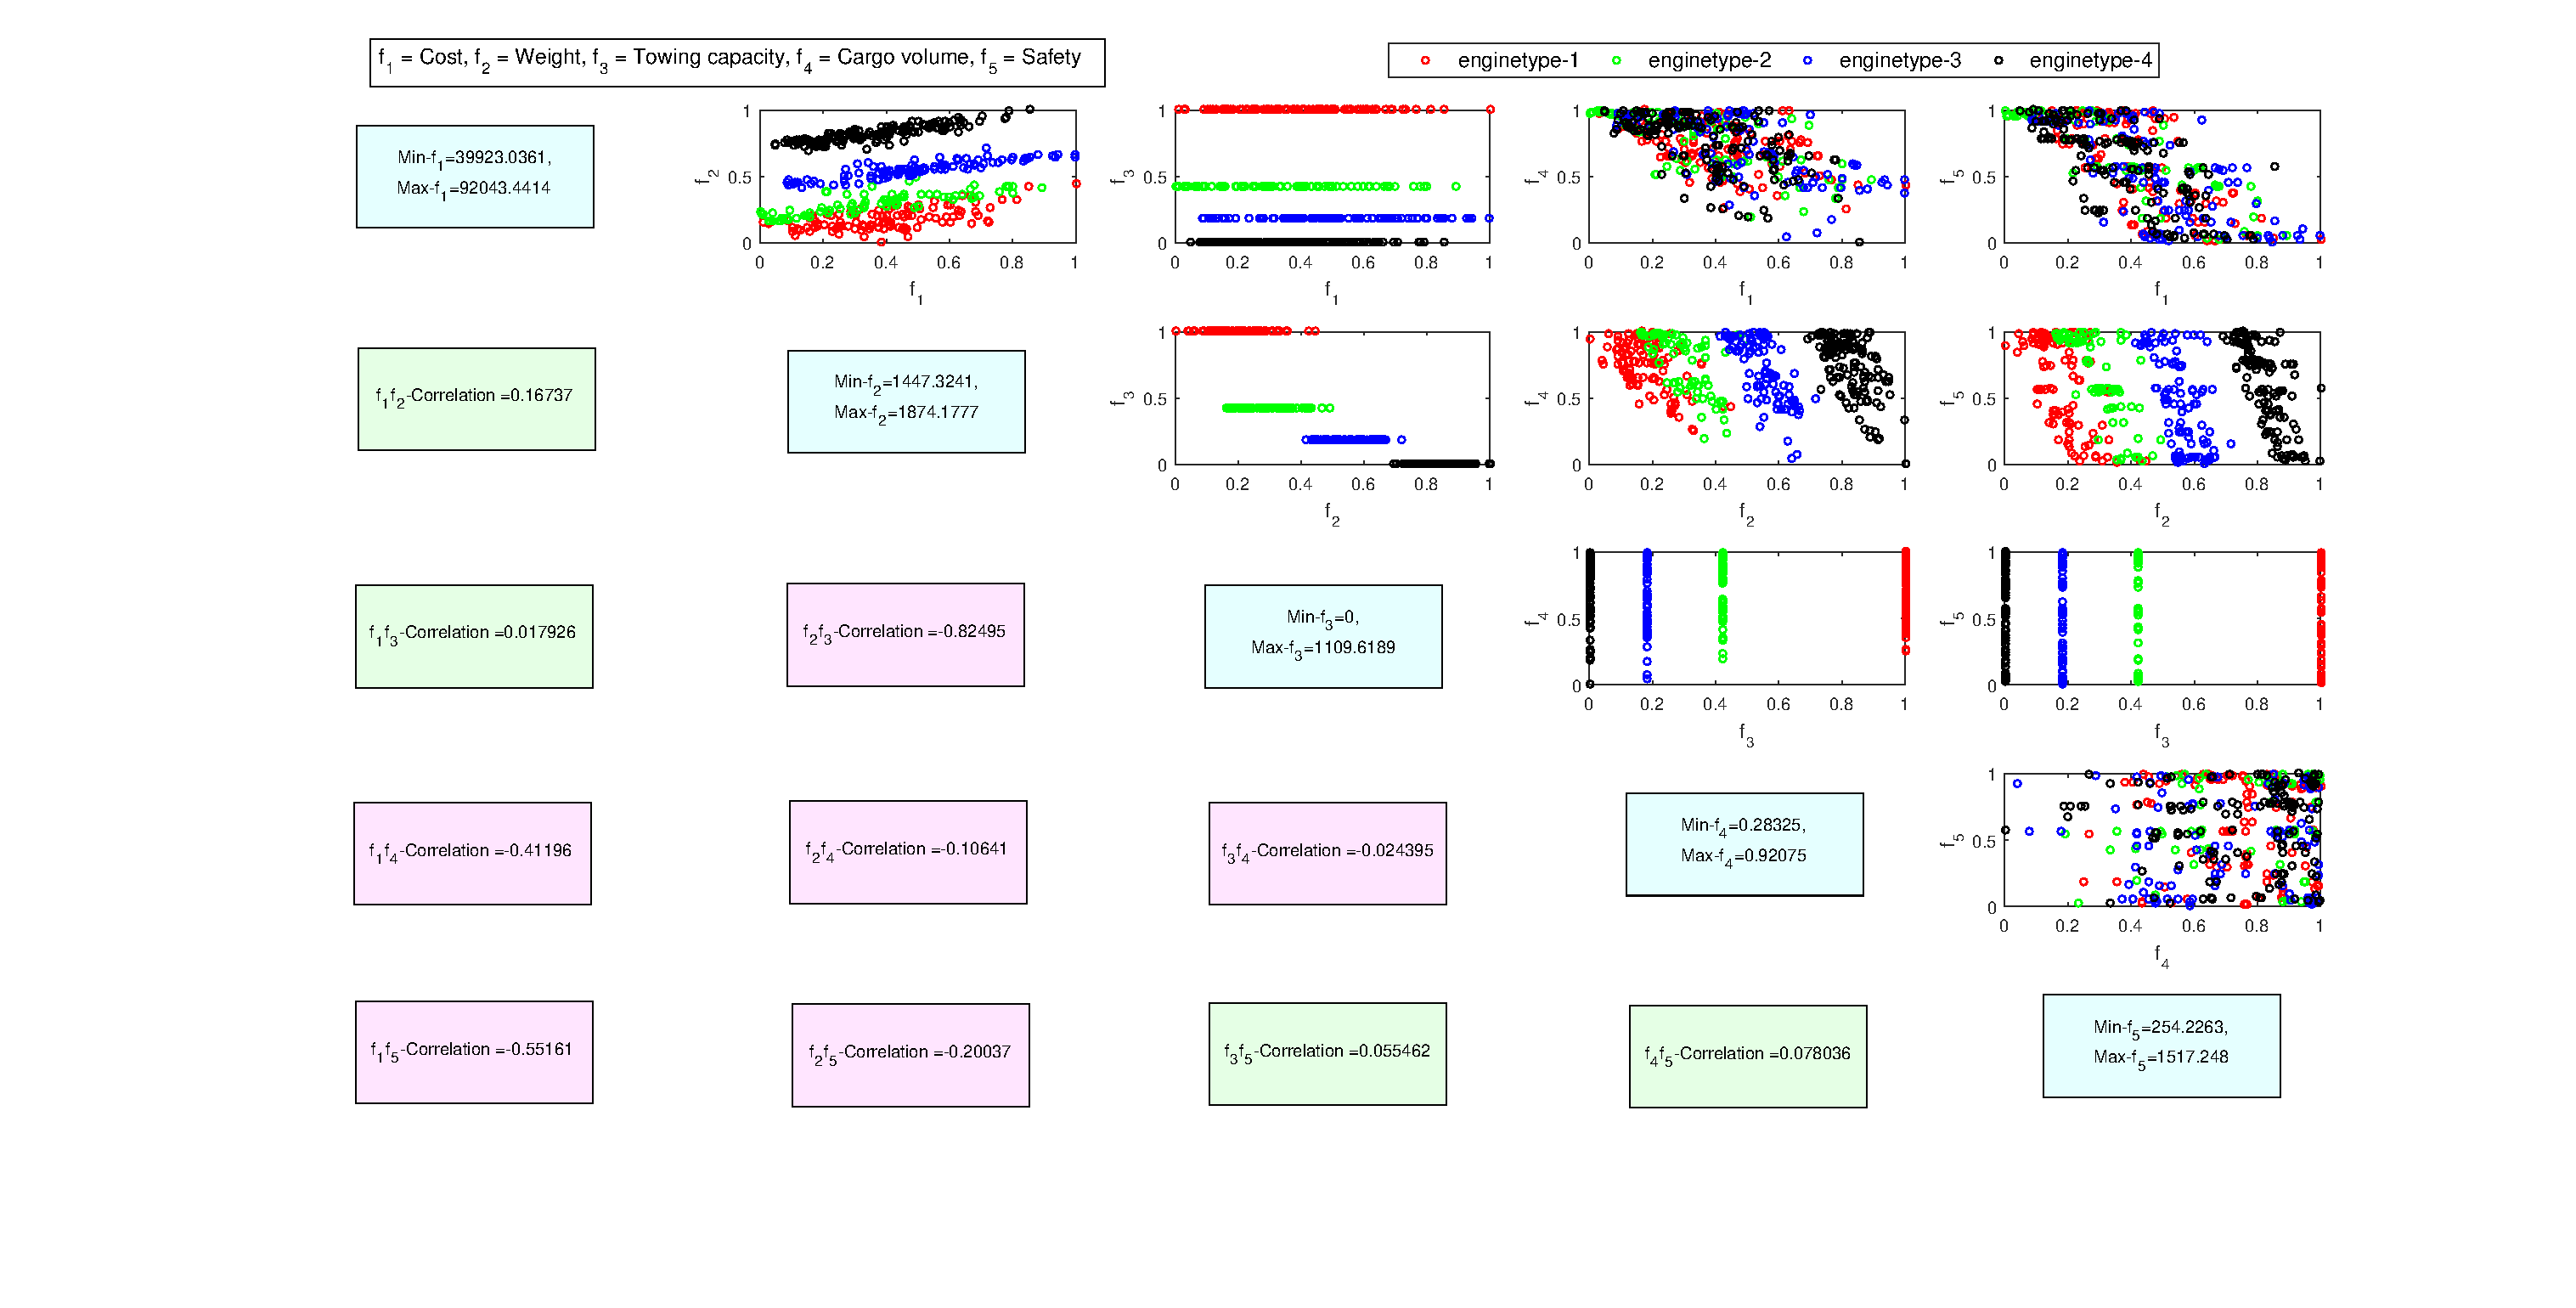
\includegraphics[scale=.21]{fig6.eps}
	\caption{Nondominated solutions for the run with the lowest IGD value for 3-objective C1DTLZ3 obtained using A-DBEA}
	\label{fig:frontc}
\end{figure}		

\subsection{Practical engineering design problems}

Lastly, we demonstrate the performance of A-DBEA on four engineering design optimization problems. Of these, first three have been used for benchmarking in some of the earlier studies, whereas the fourth one~(Wind Farm Layout) is newly formulated.  

\subsubsection{Car Side Impact}

This is a 3-objective problem with 10 inequality constraints, studied in \cite{Deb2014adaptive}. The problem aims at minimizing the weight of the car ($f_1$), the pubic force experienced by a passenger ($f_2$) and the average velocity of the V-pillar responsible for withstanding the impact load ($f_3$). The constraints represent limiting values of abdomen load, pubic force, velocity of V-pillar, (upper, middle and lower) rib deflection, velocity of front door at V-pillar. 7 design variables are considered, which correspond to the thickness of B-pillar inner, thickness of B-pillar reinforcement, thickness of floor side inner, thickness of cross members, thickness of door beam, thickness of door belt-line reinforcement and thickness of roof rail. 

The reference set containing 204,908 solutions was constructed by identifying the nondominated solutions from all solutions across all runs and available from authors' website~\cite{mdo2017adbea}. The performance of the proposed algorithm in terms of HV and IGD is shown in Table \ref{tab:hvcsiwrgaa} and compared with I-DBEA~\cite{Asafmany2015}. It is evident that based on HV and IGD metrics, I-DBEA performs worse than A-DBEA. The efficiency of the proposed approach can be accounted for having a better constraint handling strategy.	

\begin{table}[!htb]\scriptsize
	\centering
	\caption{Statistics for Car Side Impact, Water Resource Management and General Aviation Aircraft problem}
	\label{tab:hvcsiwrgaa}
	\begin{tabular}{|l|l|l|l|l|}
		\noalign{\smallskip}\hline
		\multicolumn{5}{|c|}{\textbf{Car Side Impact}}                                                 \\ \hline
		\textbf{}       & \multicolumn{2}{c|}{\textbf{HV}}      & \multicolumn{2}{c|}{\textbf{IGD}}    \\ \hline
		\textbf{}       & \textbf{A-DBEA}   & \textbf{I-DBEA}   & \textbf{A-DBEA}   & \textbf{I-DBEA}  \\ \hline
		\textbf{Best}   & \textbf{0.817511} & 0.761464          & \textbf{3.33E-02} & 6.36E-02         \\ \hline
		\textbf{Mean}   & \textbf{0.816900} & 0.738256          & \textbf{3.58E-02} & 7.89E-02         \\ \hline
		\textbf{Median} & \textbf{0.816999} & 0.741503          & \textbf{3.54E-02} & 7.79E-02         \\ \hline
		\textbf{Worst}  & \textbf{0.816168} & 0.673136          & \textbf{3.96E-02} & 1.02E-01         \\ \hline
		\multicolumn{5}{|c|}{\textbf{Water Resource Management}}                                                  \\ \hline
		\textbf{}       & \multicolumn{2}{c|}{\textbf{HV}}      & \multicolumn{2}{c|}{\textbf{IGD}}    \\ \hline
		\textbf{}       & \textbf{A-DBEA}   & \textbf{I-DBEA}   & \textbf{A-DBEA}   & \textbf{I-DBEA}  \\ \hline
		\textbf{Best}   & 0.779315          & \textbf{0.806251} & \textbf{4.56E-02} & 8.42E-02         \\ \hline
		\textbf{Mean}   & 0.771225          & \textbf{0.782277} & \textbf{4.79E-02} & 1.39E-01         \\ \hline
		\textbf{Median} & 0.770222          & \textbf{0.785335} & \textbf{4.81E-02} & 1.43E-01         \\ \hline
		\textbf{Worst}  & \textbf{0.766954} & 0.708251          & \textbf{5.06E-02} & 2.69E-01         \\ \hline
		\multicolumn{5}{|c|}{\textbf{General Aviation Aircraft}}                                       \\ \hline
		\textbf{}       & \multicolumn{2}{c|}{\textbf{HV}}      & \multicolumn{2}{c|}{\textbf{IGD}}    \\ \hline
		\textbf{}       & \textbf{A-DBEA}   & \textbf{I-DBEA}   & \textbf{A-DBEA}   & \textbf{I-DBEA}  \\ \hline
		\textbf{Best}   & 0.07331           & \textbf{0.08553}  & 0.23540           & \textbf{0.20677} \\ \hline
		\textbf{Mean}   & 0.06533           & \textbf{0.07357}  & 0.26899           & \textbf{0.22817} \\ \hline
		\textbf{Median} & 0.06556           & \textbf{0.07436}  & 0.26745           & \textbf{0.22269} \\ \hline
		\textbf{Worst}  & 0.05469           & \textbf{0.05670}  & 0.32226           & \textbf{0.27741} \\ \hline
	\end{tabular}
\end{table}

\subsubsection{Water Resource Management}

This is a 5-objective problem with 7 constraints. The formulation of the problem was originally introduced in \cite{musselman1980water} and has been studied subsequently studied in a number of works~\cite{Ray2001,asaf2012manyeps,Asafmany2015}.  For this problem, HV and IGD computations are based on the nondominated solutions obtained from the accumulated final populations of all optimization runs.

IGD value is computed using the targeted reference set of 6725 nondominated solutions instead of the reference set reported in \cite{durillo2011jmetal} which had  2429 solutions. Although all 2429 solutions are members of 6725 reference solutions, our algorithm identified some solutions with lower objective values than the ideal vector of the reference set~\cite{durillo2011jmetal}. Hence we created a combined ND set obtained from all 21 runs and the reference set provided in \cite{durillo2011jmetal}. The clear differences in ideal and nadir is marked in bold in Table \ref{tab:prob_param}. The performance of the proposed algorithm in terms of HV and IGD values is presented in Table~\ref{tab:hvcsiwrgaa} and compared with I-DBEA. While performance in terms of HV is better for I-DBEA it suffers in terms of IGD compared to A-DBEA. While I-DBEA relies only on global nondominance during replacement, A-DBEA also focuses on diversity of the solutions which has resulted in better IGD measure. With better constraint handling strategy, better extremal solutions were identified, especially with lower values of the second objective~(around 11.8164 units better than the second objective value of the ideal vector of the 2429 dataset). The current nadir vector is extended by approximately 259.4326 units in the first objective, 2.6468$\times 10^4$ units in the fourth objective and 219.3600 units in the last objective value compared the nadir vector of the 2429 dataset. The new reference set is now made available for download from the authors' website~\cite{mdo2017adbea}. 


\subsubsection{General Aviation Aircraft}

This problem was first introduced in \cite{Simpson1996} and has been solved using an evolutionary algorithm in \cite{Hadka2012many}. The problem involves 9 design variables: cruise speed, aspect ratio, sweep angle, propeller diameter, wing loading, engine activity factor, seat width, tail length/ diameter ratio and taper ratio and the aim is to minimize the takeoff noise, empty weight, direct operating cost, ride roughness, fuel weight, purchase price, product family dissimilarity and maximize the flight range, lift/ drag ratio and cruise speed. Previous studies have encountered difficulties in obtaining feasible solutions due to tight constraints~\cite{Simpson1996}. For this problem, HV and IGD computations are based on the nondominated solutions obtained from the accumulated solutions from all optimization runs.

IGD value is computed using the targeted reference set of 5217 nondominated solutions instead of the reference set of 530 nondominated solutions obtained using $\epsilon$-MOEA and Borg-MOEA from \cite{Hadka2012many}. Although all 530 nondominated solutions are members of the 5217 reference solutions, our algorithm identified some solutions with higher objective values than the nadir vector of the reference set\cite{Hadka2012many}. The updated objective values of the nadir vector is marked in bold in Table~\ref{tab:prob_param}. With better constraint handling strategy, better extremal solutions were identified, especially with higher values of the first objective~(around 0.0428 units better than the first objective value of the nadir vector of 530 dataset), fifth objective~(around 10.7739 units better than that of 530 dataset) and last objective~(around 0.3663 units better than that of 530 dataset). The new reference set is now made available for download from the authors' website~\cite{mdo2017adbea}. The performance of the proposed algorithm is presented in Table~\ref{tab:hvcsiwrgaa} and compared with I-DBEA~\cite{Asafmany2015}. The targeted reference set was constructed using a combined nondominated set of solutions obtained from all the solutions evaluated in 21 runs (of both I-DBEA and A-DBEA) and the reference set is provided in \cite{Hadka2012many}. Similar strategy of performance comparison were followed for both the approaches. Performance of I-DBEA is better in terms of both HV and IGD in this problem possibly due to having global nondominance during replacement. 

\subsubsection{Wind Farm layout optimization problem}


\begin{figure*}[!htb]
	\centering
	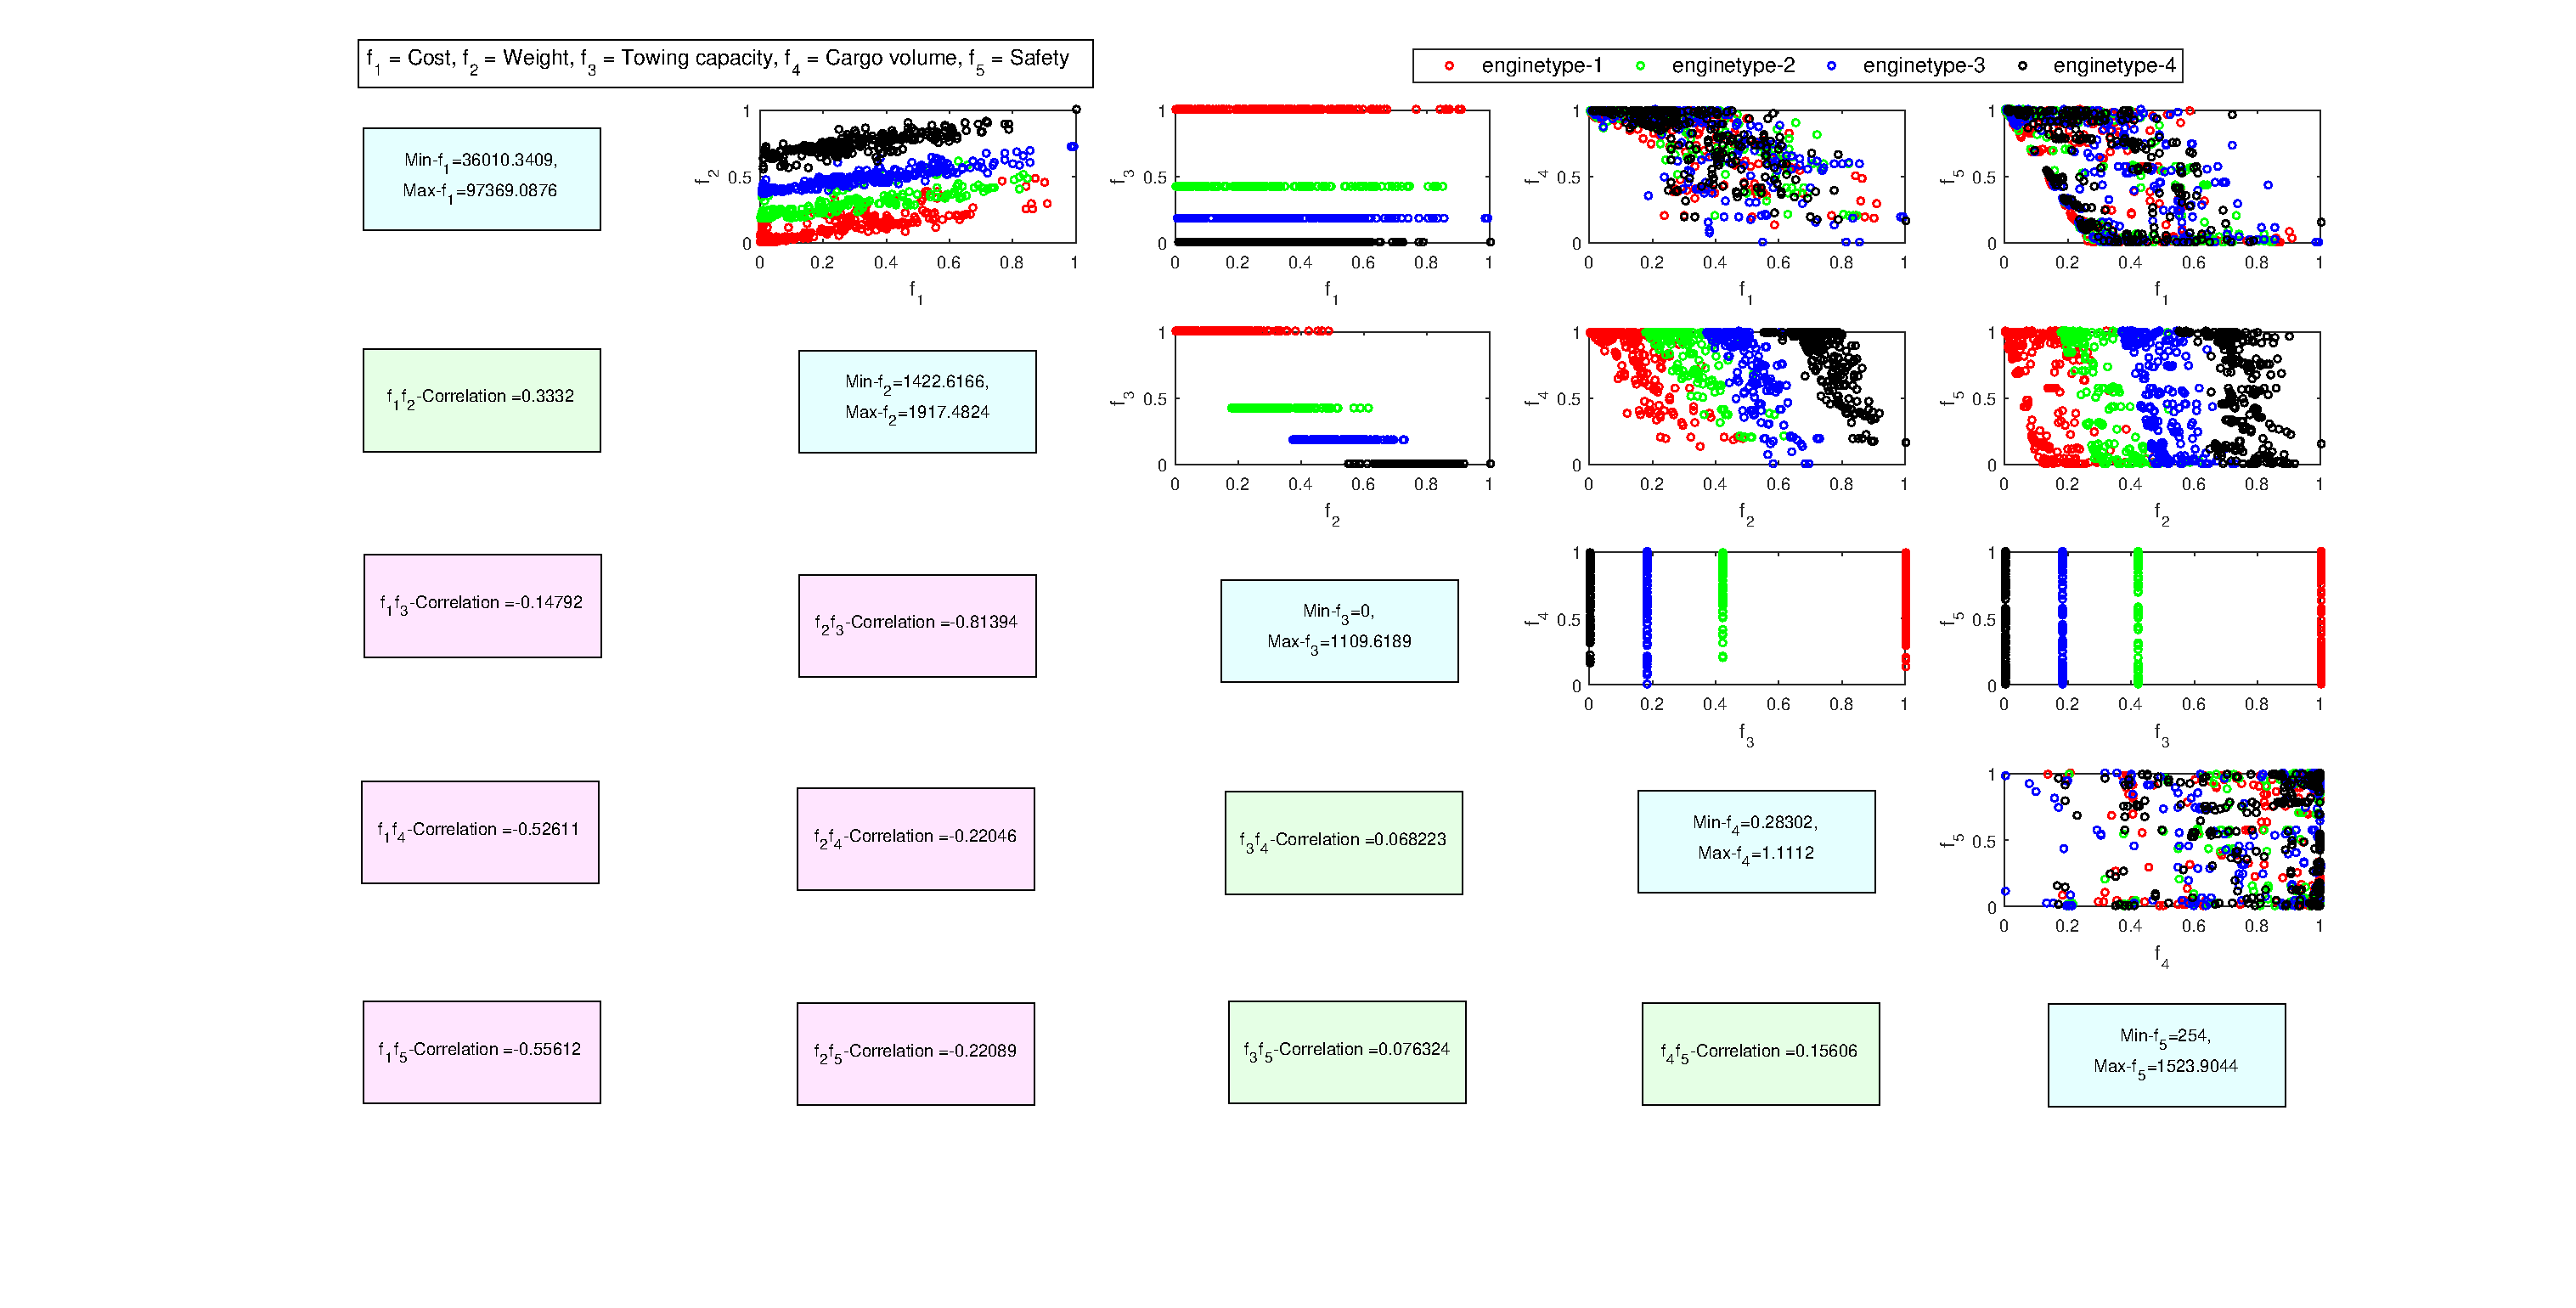
\includegraphics[scale=.35]{fig7.eps}
	\caption{Wind farm layouts corresponding to the best value in each objective} 
	\label{fig:layouts}
\end{figure*}

Wind is one of the most promising sources of alternative energy. This problem presents a model for optimum wind turbine placement within a landmass with irregular boundaries. Objectives include maximization of wind power, minimization of cable length connecting the turbines, minimization of enclosed land area~(associated with inspection and maintenance) and minimization of the noise level. In a vast majority of the studies, the problem is modeled as a power maximization problem by minimizing wake effect~(i.e. inter turbine interaction)~\cite{kusiak2010wind,chowdhury2012uwflo,turner2014mp}. There are also attempts to model it as a bi-objective optimization problem, i.e., minimization of noise level~\cite{tran2013mowind,kwong2014mo,sorkhabi2016mo} in addition to maximization of the wind power. Considerations of irregular land geometry have also been suggested\cite{gu2013irre,song2013terr}. In this study, we present a more realistic formulation of the problem with practical considerations and complexity. These include (a) irregular land geometry (b) multiple irregular infeasible regions where turbines cannot be placed due to environmental regulations~(archaeological deposits, bird feeding areas, natural flora, water bodies etc.) (c) statutory requirements on noise levels for nearby residential dwellings. The objective is to place 30 wind turbines while considering (a) maximization of power generation (b) minimization of noise level at the residential dwellings~(must be less than 40 dB(A) as per the regulations~\cite{SPA2009}) (c) minimization of convex hull area in which turbines are placed and (d) minimization of the cabling length~(for cost reduction). The wind distribution is identical to the wind scenario-2 in~\cite{kusiak2010wind}. The noise calculation is based on \cite{isonoise,kwong2014mo,stdaus2010,sorkhabi2016mo} and the parameters related to the proximity constraint threshold, spread, rated power are identical to \cite{kusiak2010wind}.  


To solve this problem, the allowable feasible land is discretized into 3622 triangles using Delaunay triangulation, and each triangle comprises 8001 locations generated using NBI approach~\cite{das1998normal}. This is done in order to avoid infeasible layout configurations. The cabling layout is also considered within the allowable feasible land only and based on minimum spanning tree. However, if a cable connecting two turbines passes through the infeasible regions/crosses the boundary of the irregular allowable land, it is rerouted. The location of a turbine can be represented using the identity of the triangle and the identity of a point within the triangle.

From the optimization run, the algorithm was able to identify 393 nondominated solutions. The maximum power, minimum cable length, minimum land area and minimum noise level achieved were 3.686 MW, 1.126$\times 10^4$ m, 4.814$\times 10^6$ m\textsuperscript{2} and 35.475 dB(A) respectively. Among the feasible solutions there were variations of 3.18 \%, 37.99\%, 62.53\% and 22.60\% in terms of power generation, cable length, land area and noise level respectively. The turbine layouts corresponding to best values in each objective are shown in Fig.~\ref{fig:layouts} and the noise profile on the residential areas corresponding to each scenario are also indicated. For example, one can clearly observe that turbines corresponding to minimum noise level are far away from the residential area and the noise profile on the residential area indicates lower values of noise compared to the other three situations. One can also observe that there can be about 3\% improvement in power generation, while improvements in other objectives could be much more significant. Therefore, dealing this problem as a many-objective optimization problem offers the opportunity to identify better trade-off solutions as opposed to dealing it as a single-objective problem of power maximization.    

\section{Summary and Conclusions}
\label{sec:sum}

In this paper we have presented a novel approach to deal with multi/many-objective optimization problems and illustrated its utility to deal with practical engineering optimization problems. The novel aspects include: (a) the use of layered assignment-only scheme that eliminates need for additional schemes for replacement and preserves diversity while maintaining good convergence; (b) the strategy does not enforce strict nondominance for assignment, and thus is able to deal with deceptive problems were a part of the Pareto front may be obtained significantly sooner than others; (c) preservation of infeasible solutions to promote search around constraint boundaries; and (d) use of alternating crossover strategies between DE and SBX to capitalize on their individual benefits.  

The performance of the algorithm was benchmarked against state-of-the-art algorithms using on several problems. The results indicate that the algorithm performs well on all problems based on HV and IGD measures. Furthermore, for both the constrained practical problems~(Water Resource Management and General Aviation Aircraft problem), the algorithm identified better extremal solutions than known previously. This can be attributed to better constraint handling strategy combined with extremal solution identification scheme via the achievement scalarizing function. Finally, we introduce a four objective Wind Farm Layout optimization problem involving irregular land boundaries and infeasible areas, with noise and proximity constraints. This in our opinion is a close to real-life formulation of the problem that can be used to assess performance of constrained many-objective optimization algorithms.

In this study, we have used a fixed set of reference directions during the search. Further improvement in generalization and efficiency can be achieved by considering (a) reference directions both from nadir and ideal and (b) adaptive addition/deletion of these reference directions. These are some of the the current research directions pursued by the authors.  


 






